\section{Introduction}
In many contexts (e.g. industry, academic research, etc.), users want to get insights about their data. In such cases, the number of variables (or \emph{features}) characterizing each element (or \emph{instance}) in their database (or \emph{dataset}) is often too large to understand their data. The problem of {\it dimensionality reduction} is to reduce a dataset containing $d$ features for $n$ instances (providing an $n \times d$ matrix) to a new dataset containing significantly less features. When this new number of features equals two, the dimensionality reduction result allows users to see their data in a two-dimensional space by plotting the remaining two features in a scatter plot. This problem is called {\it visualization}: from provided data with too many features, visualization algorithms provide a projection of these data in a two-dimensional space in such a way that the information loss is minimized. The resulting $n \times 2$ matrix, often called {\it embedding}, can then be visualized using a scatter plot.
Fig.~\ref{subfig:digit_viz_example} represents a 2D scatter plot visualization of 200 hand-written digits images and Fig.~\ref{subfig:digit_example} shows some examples of the raw image data.

%% \begin{figure}
%%     \centering
%%     \begin{subfigure}[c]{0.43\linewidth}
%%         \frame{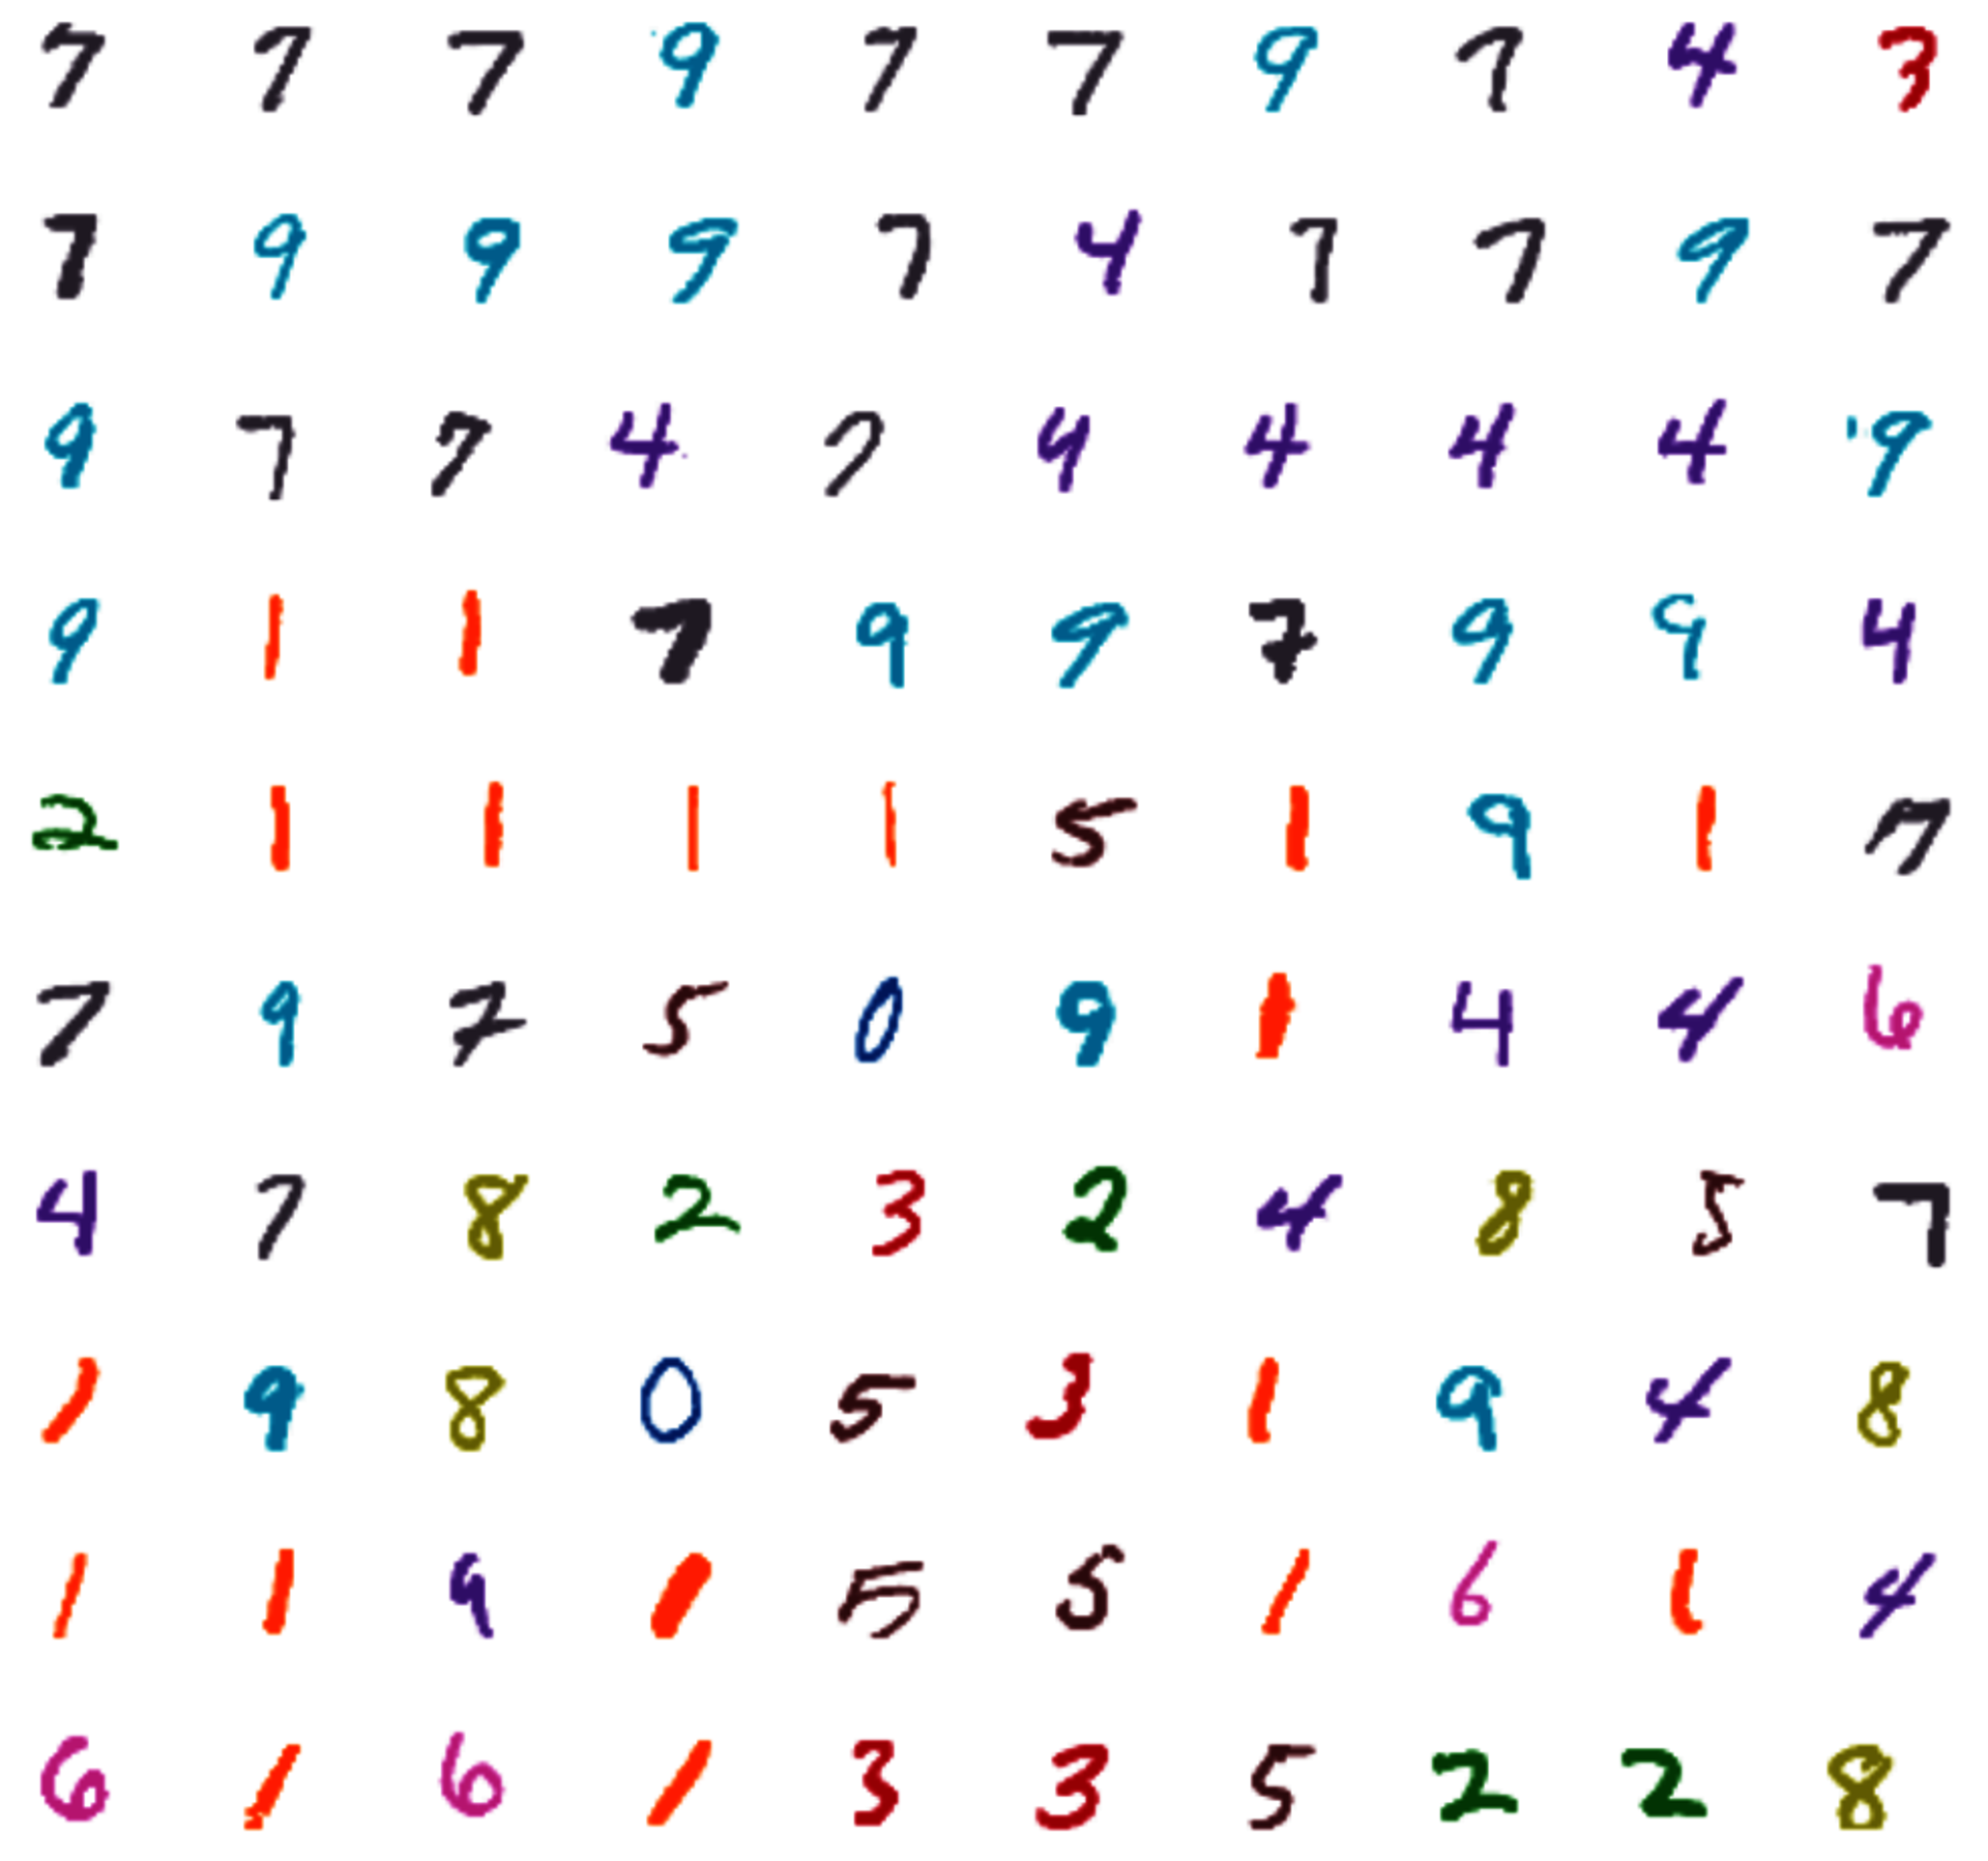
\includegraphics[width=\textwidth]{mnist_raw200}}
%%         \caption{Examples of hand-written digit images.}
%%         \label{subfig:digit_example}
%%     \end{subfigure}
%%     \begin{subfigure}[c]{0.55\linewidth}
%%         \frame{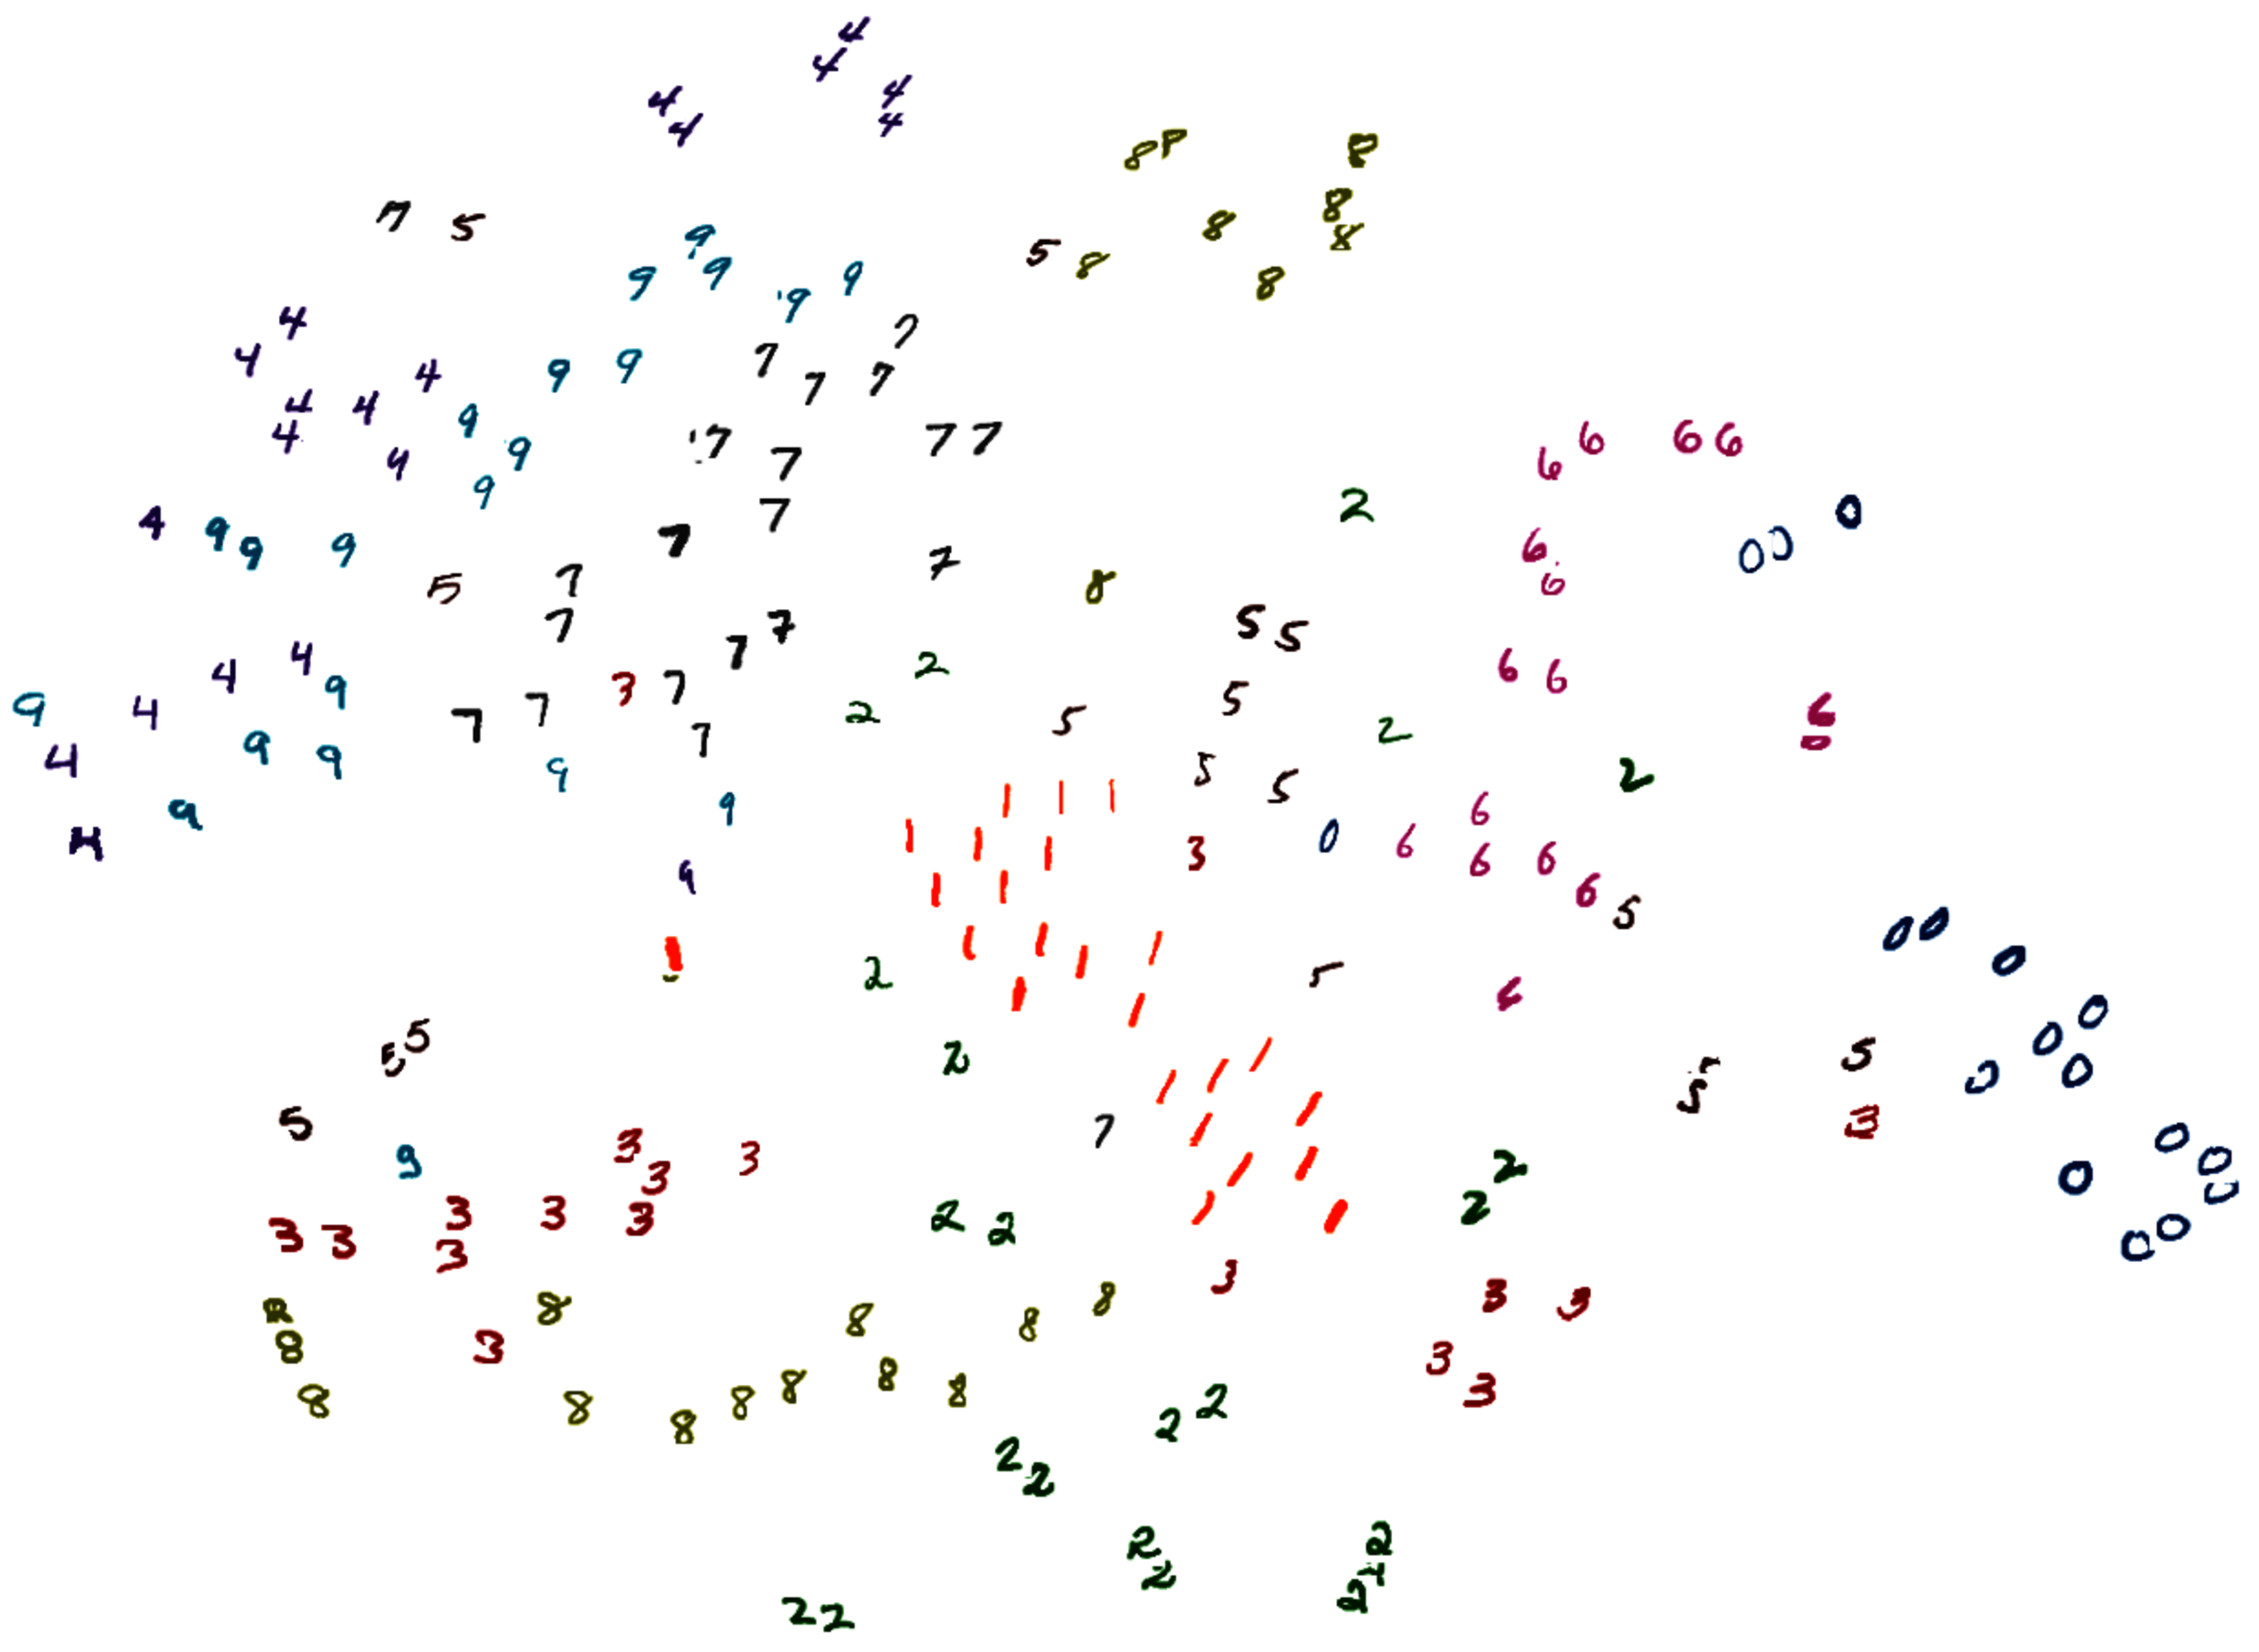
\includegraphics[width=\textwidth]{mnist_viz200}}
%%         \caption{A visualization created by \mbox{$t$-SNE}.}
%%         \label{subfig:digit_viz_example}
%%     \end{subfigure}
%%     \caption{Example of 32x32 images of hand-written digits which are visualized by a dimensionality reduction technique ($t$-SNE) and represented in a 2D scatter plot.}
%%     \label{fig:dr_viz}
%% \end{figure}

Among the available visualization algorithms, some require to tune one or more parameters (called {\it hyperparameters}). This step is crucial, since it predetermines the quality and usefulness of the obtained visualization. Typically, the desired visualization result has to be chosen through trial and error by the user among all generated results using different hyperparameter values. This process is tedious and it is difficult for the user to find the best suiting visualization.

\begin{figure*}
  \centering
  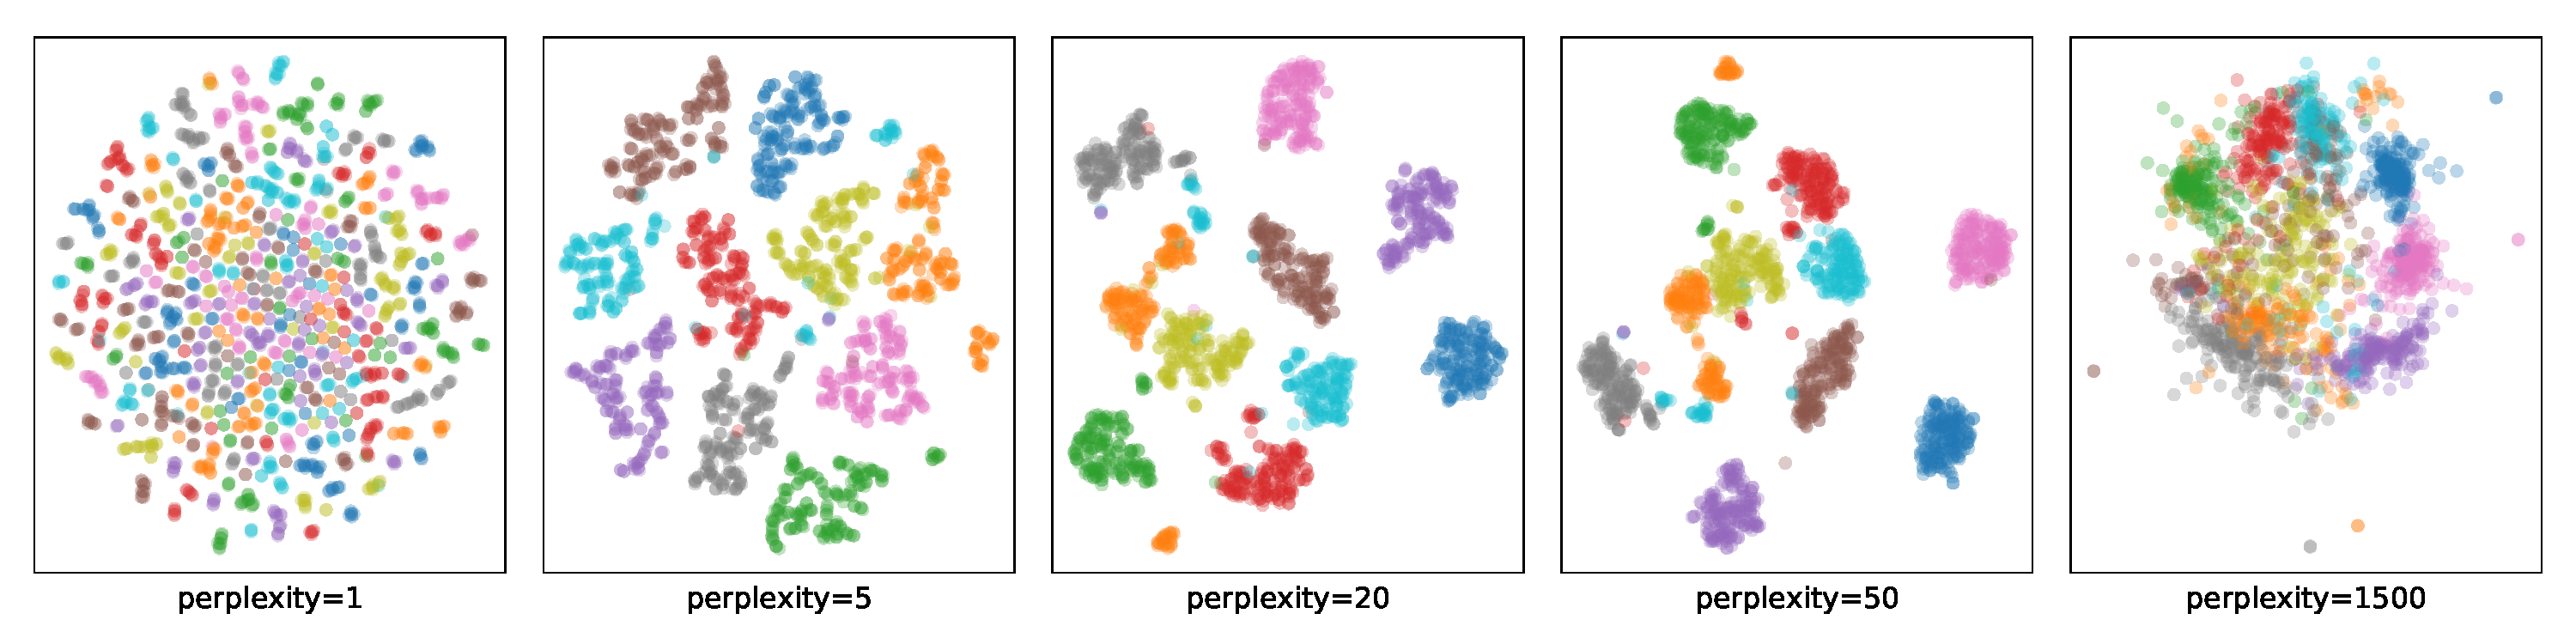
\includegraphics[width=\linewidth]{MNIST-SMALL_examples}
  \caption{Visualization of the \emph{DIGITS} dataset by $t$-SNE with five different perplexity values preserving from local (left) to global (right) topology of the dataset. The dataset contains 1797 gray-scale 8x8 images of ten handwritten digits. The colors correspond to the digit labels. Obtaining compact clusters (perplexities of 20 and 50) is usually considered better.}
  \label{fig:mnist_perps}
\end{figure*}

%%%%%%%%%%%%%%%%%%%%%%%%%%%%%%%%%%%%
In this paper, we show how to automatically choose one of the hyperparameters of $t$-distributed Stochastic Neighbor Embedding ($t$-SNE)~\cite{maaten2008tsne}, the {\it perplexity}, by considering user constraints.
The perplexity, detailed in subsection \ref{subsec:perplexity}, is a measure of the compromise between global or local structure preservation during the dimensionality reduction process.
We propose to consider user constraints on the dataset of interest to maximize the chance for the most suitable visualization to be presented to the user.
The constraints are in form of relationships between object pairs, which are easier to express and understand.
These user pairwise constraints are first transformed into a quantitative measure called \emph{constraint-preserving score}.
This score is then used to find the best perplexity hyperparameter of $t$-SNE corresponding to the best visualization that respects the user needs.
Based on this idea, our work is driven by the main research question: is the constraint-preserving score reliable and how good are visualizations with respect to well-known visualization quality metrics?

%{\bf [RQ1]} What are the characteristics of the constraint-preserving score that help us find the best perplexity?

%{\bf [RQ2]} Is the constraint-preserving score reliable and how good are visualizations with respect to well-known visualization quality metrics?

%{\bf [RQ3]} How are the visualizations of the best embeddings selected using our proposed method and the visualization quality metrics?


This paper is organized as follows. Section \ref{sec:background} presents the background on dimensionality reduction, visualization and $t$-SNE. Section \ref{sec:related_work} provides an overview on how the perplexity is handled in the literature as well as the usage of constraints in clustering and dimensionality reduction methods.
Our proposed method, which takes user constraints into account in order to select the perplexity, is introduced in Section~\ref{proposed_method}. The experimental setting for evaluating the proposed method is described in Section \ref{XP}. The results that allow us to answer the presented research question are shown in Section \ref{sec:results}. Finally, Section \ref{sec:ccl} concludes our work.

%%%%%%%%%%%%%%%%%%%%%%%%%%%%%%%%%%%%%%%%%%%%%%%%%%%%%%%%%%%%%%%%%%%%%%%%%%%%%%
\section{Dimensionality Reduction and $t$-SNE}\label{sec:background}

Dimensionality reduction (DR) is an unsupervised learning problem in machine learning with the goal of reducing the number of dimensions of a multivariate dataset while preserving its important characteristics. Typical characteristics that DR techniques try to preserve are variances (as in PCA), similarities and distances between objects (distance-preserving, as in MDS), or cluster structures and neighborhood information among objects (neighborhood-preserving, as in $t$-SNE) \cite{lee2007}.

$t$-distributed Stochastic Neighbor Embedding ($t$-SNE)~\cite{maaten2008tsne}, one of the most widely used DR method, preserves the neighborhood information by creating an embedding in such a way that the points that are neighbors in the original high-dimensional space (HD) will still be neighbors in the reconstructed low-dimensional space (LD).
The number of neighbors to consider for each point (controlled by the \emph{perplexity} hyperparameter) is usually determined by users.
Fig.~\ref{fig:mnist_perps} shows some visualizations generated with different perplexities.
We can see that the structure in each visualization changes according to the considered number of neighbors for each point, defined by the perplexity.
When the perplexity is very small, small local groups/clusters of points appear. These groups become more and more large and compact when the perplexity increases, meaning that we consider the preservation of more neighbors for each point.
However, when the perplexity is too large, each point is considered as neighbor of every other point, which leads to a crowded ball-shaped cluster.
This evolution is a specific characteristic of $t$-SNE and of the neighborhood-preserving DR methods in general.
In order to use $t$-SNE efficiently, the user is required to have a good knowledge of the dataset for choosing a reasonable perplexity as well as for interpreting and analyzing the visualization.

The goal of $t$-SNE is to preserve the topology expressed by the neighborhood information.
Unfortunately, this information is not given explicitly and requires the computation of the distance between each pair of points in the dataset. 
In the literature, the classical distance-preserving DR techniques are not efficient since they can not fully retain both global and local structure of the high dimensional data \cite{maaten2008tsne, van2009comparativeReview}.
$t$-SNE tackles this problem by transforming the pairwise distances in HD and LD into probabilities.

The intuition behind this probability-preserving approach is as follows.
Let us assume that the original data in HD is modeled by a distribution $P$ and the reduced data in LD is modeled by a distribution $Q$.
These two distributions represent the probability of being neighbors for each pair of points in HD and LD, respectively.
The goal is to change the target embedding producing $Q$ in such a way that $Q$ is as close to $P$ as possible.
The \emph{closeness} between these distributions is measured by the \emph{Kullback-Leibler (KL) divergence}.
The objective of $t$-SNE is to minimize a measure called the \emph{KL loss}, by seeking an embedding whose distribution $Q$ comes closer and closer to the true distribution $P$ \cite{maaten2008tsne}:

\begin{equation}\label{eq:p_j|i}
    p_{j|i} = \frac{\textnormal{exp}(-||x_i - x_j||^2/2\sigma_i^2)}{\sum_{k\not=i}\textnormal{exp}(-||x_i - x_k||^2/2\sigma_i^2)}
\end{equation}

\begin{equation}
    p_{ij} = \frac{p_{j|i}+p_{i|j}}{2}
\end{equation}

\begin{equation}\label{eq:q_ij}
    q_{ij} = \frac{(1+||y_i - y_j||^2)^{-1}}{\sum_{k\not=l}(1+||y_k - y_l||^2)^{-1}}
\end{equation}

\begin{equation}\label{eq:KL}
    KL(P||Q) = \sum_{i}\sum_{j} p_{ij} \textnormal{log}\frac{p_{ij}}{q_{ij}}
\end{equation}

$t$-SNE is controlled by the perplexity which approximates the number of neighbors considered for each point through $\sigma$ in Eq.~\ref{eq:p_j|i}. The user can change the perplexity, the most important $t$-SNE hyperparameter, to obtain different visualizations.
With a small perplexity, the local structure is preserved, while a larger perplexity pays more attention to the global structure of the dataset.
Tuning this parameter is a difficult task and is often done by trial and error.
For facilitating this process, some techniques exist for choosing a good perplexity, as shown in the next section.

\section{Related Works}\label{sec:related_work}
This section first reviews the problem of selecting the perplexity, an important hyperparameter of $t$-SNE. We show why choosing a good perplexity is still a hard problem and present some existing solutions in Section \ref{subsec:perplexity}.
As our proposed method is based on user pairwise constraints, we quickly review their usage in clustering and dimensionality reduction methods in Sections \ref{subsec:constraints_clustering} and \ref{subsec:constraints_dr}.

\subsection{Choosing a Good Perplexity for $t$-SNE}
\label{subsec:perplexity}

The right perplexity to choose depends on the characteristics of the dataset such as the number of instances (size), the topology (structure) or the density (distribution) of instances, which makes it hard to select the best one.
The original paper of van der Maaten et al. \cite{maaten2008tsne} suggests typical values between 5 and 50.
However, in practice, the embedding can change drastically between two different perplexity values. Therefore, there is no evidence to ensure that the suggested perplexities are good for all datasets.
The original paper also proposes a simple method to select a good perplexity by looking at the KL loss produced by several perplexities and choose the lowest one, since it corresponds to a well-preserved neighborhood.
However, the KL loss tends to naturally decrease when the perplexity increases \cite{cao2017automatic}, which  is confirmed by our experiments as shown in Fig.~\ref{fig:klloss}. For this reason, it is unsuitable to use the KL loss for evaluating the embedding quality since a very high perplexity would be chosen.

\begin{figure}
    \centering
    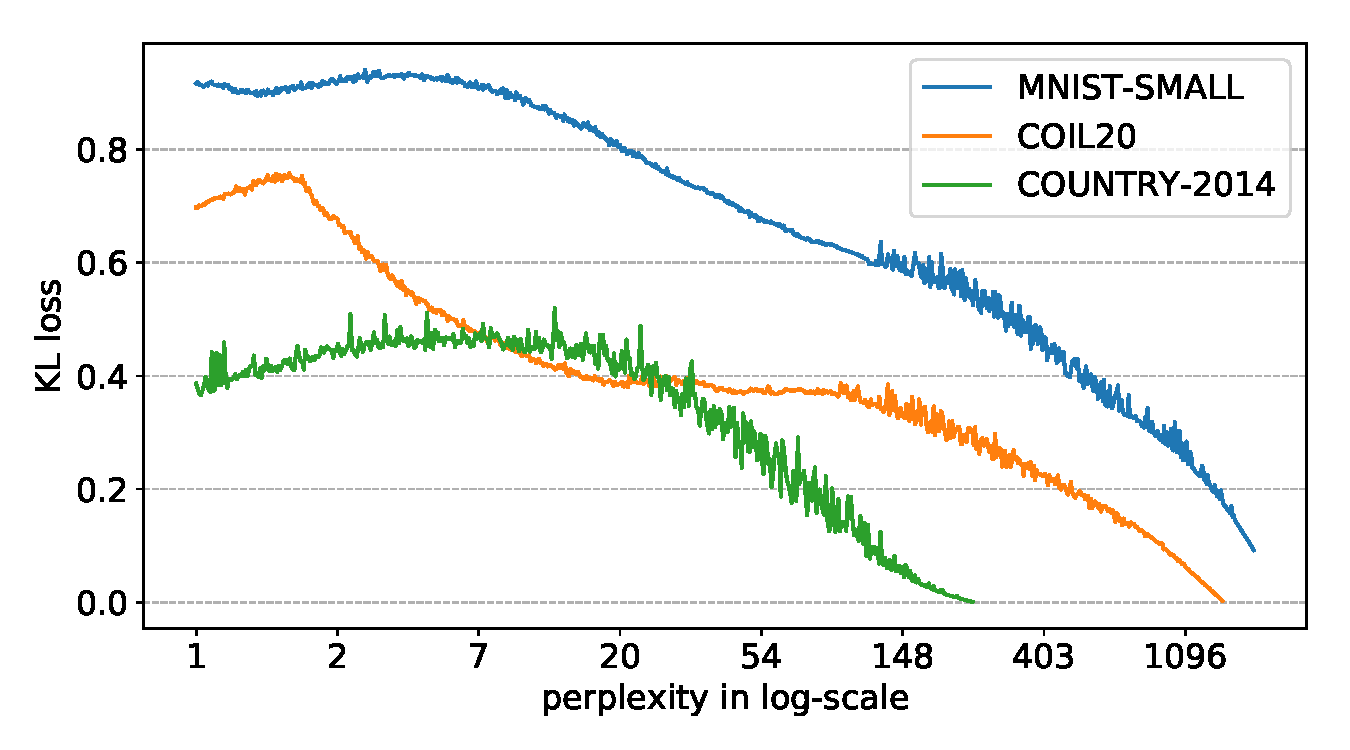
\includegraphics[width=0.95\linewidth]{klloss_all}
    \caption{For three different datasets, the KL loss tends to decrease when the perplexity increases. Note that the values of KL loss across different datasets are not comparable.}
    \label{fig:klloss}
\end{figure}

In practice, users have to carefully choose a hard-to-understand perplexity to obtain a good embedding result.
Even though this process requires an expertise in machine learning, it is often tedious and error-prone.
Our idea is to let users suggest \emph{how close instances have to be in the visualization} by using constraints, in order to propose the most suitable visualization for them.

Few papers in the literature attempt to derive the best perplexity automatically.
Strickert~\cite{strickert2012} evaluates the degree of neighborhood P*, instead of P, by using a given pairwise score matrix S. For each instance $i$ in ${\bf S}$, all other instances $j$ are ranked and {P*}$_{ij}$ is computed with respect to the ranking position of each instance $j$ in ${\bf S}_i$. However, this solution is not suitable when the matrix ${\bf S}$ is not provided.
Lee et al.~\cite{lee2014} use a multi-scale approach by considering, and averaging, all neighborhood sizes. Despite providing visualizations by bypassing the perplexity selection problem, Lee et al. do not offer a solution for the selection problem itself.
On the contrary, Cao and Wang~\cite{cao2017automatic} select the perplexity that minimizes the modified \emph{Bayesian Information Criteria} (\emph{BIC}):
\begin{equation}
S(\textit{perplexity}) = 2KL(P||Q) + \log(n)\frac{\textit{perplexity}}{n},
\end{equation}
where $KL(P||Q)$ is the same KL loss as Eq.~\ref{eq:KL} and $n$ is the number of instances.
Their approach is validated with user-based experiments by comparing the automatically selected visualization to the ones selected by users. They obtain resultant perplexities very close to the user consensus for three datasets. The comparison between this \emph{BIC}-based approach and our proposed method is presented in Section~\ref{subsec:result_compare}.

\subsection{User Constraints for Clustering}
\label{subsec:constraints_clustering}

Clustering is a machine learning problem in which the goal is to find groups (called \emph{clusters}) of instances in the data. The constraints used in clustering methods have been well studied for a long time. User constraints can incorporate domain expertise with the goal of explicitly defining the property of the expected clusters.
The popular survey by Davidson et al.~\cite{Davidson2007surveyClt} focuses on \emph{constraint-based} and \emph{distance-based} clustering methods with instance-level constraints.
In constraint-based methods, the clusters are formed in such a way that the given constraints are preserved as much as possible, e.g. PCKMeans \cite{basu2004active} or a modified version of K-Means with feasibility under $\delta-$, $\epsilon-$ and pairwise constraints \cite{davidson2005clustering}.
In distance-based methods, the constraints are first used to train a distance function that is later used by a clustering algorithm, e.g. relation component analysis as distance measure \cite{bar2003learning} and constraint metric K-Means \cite{xing2003distance}.

The pairwise constraints are first introduced in constrained K-Means by Wagstaff et al. \cite{wagstaff2001constrained} for clustering GPS data. Must-link and cannot-link constraints indicate that two instances must be in the same cluster or cannot be in the same cluster, respectively.
In this paper, these terms are generalized for more widely usages. A similar-link constraint suggests that two points should be close or similar and a dissimilar-link constraint means that two points should be far apart or dissimilar.

\subsection{User Constraints for Dimensionality Reduction}\label{subsec:constraints_dr}
One application of user constraints in DR methods is for visualizing data in which we can inject constraints to force the output embedding to have some expected properties.
The \emph{objective constraints} can be partial labels (as in semi-supervised LDA \cite{Sugiyama2008SELF}) or constraints on the value of features (e.g. bounded PCA \cite{giordani2007bpca}). 
If users can interact with the visualization result, they can give their feedbacks in form of instance-level \emph{subjective constraints}.
Integrating user interaction into DR methods is reviewed by Sacha et al.~\cite{Sacha2017Interaction} and by Endert et al. in a wider survey on integrating machine learning into visual analysis~\cite{Endert2017SOTA}.
Pairwise constraints from user feedbacks are used to attract points connected by similar-links and repulse dissimilar-link-constrained points. Such constraints are used in e.g. pairwise constraints-guided feature projection~\cite{tang2007pairwise}, semi-supervised DR~\cite{zhang2007ssdr}, graph-driven constrained DR via linear projection~\cite{davidson2009gcdr} and constrained locality preserving projections~\cite{cevikalp2008CLPP}.

In this work, we introduce a different usage of pairwise constraints: users define subjective requirements under their personal point of view in form of pairwise constraints and the visualization hyperparameter that best fits these constraints is selected.
The constraints are not integrated in the objective function of a dimensionality reduction method.
Instead, they are used as an external measurement to evaluate the quality of the embedding in order to select the one that best matches the constraint requirements.


%%%%%%%%%%%%%%%%%%%%%%%%%%%%%%%%%%%%%%%%%%%%%%%%%%%%%%%%%%%%%%%%%%%%%%%%%%%%%%
\section{Proposed Perplexity Selection Method}\label{proposed_method}

We propose a method for automatically choosing the most appropriate perplexity for $t$-SNE.
Users define their needs in a natural manner by picking certain pairs of similar or dissimilar instances. Among all possible embedding solutions, our method chooses the one that satisfies the user pairwise constraints the most and, therefore, fits the user needs.

\subsection{Visual Definition of User Pairwise Constraints}

Since humans are capable of well distinguishing similar and dissimilar high-dimensional objects with prior knowledge (e.g. comparing countries only by their name, compare images by the visual features such as the shape, color, objects on image, etc.), they can naturally express their cognitive requirements by defining several links between instances.
In Fig.~\ref{fig:ml_cl_examples}, several examples are provided of similar-links that can be formed between objects between very similar objects under different point of view while the dissimilar-links would be formed between objects of different shapes.

\begin{figure}
    \centering
    \begin{subfigure}[c]{0.48\linewidth}
        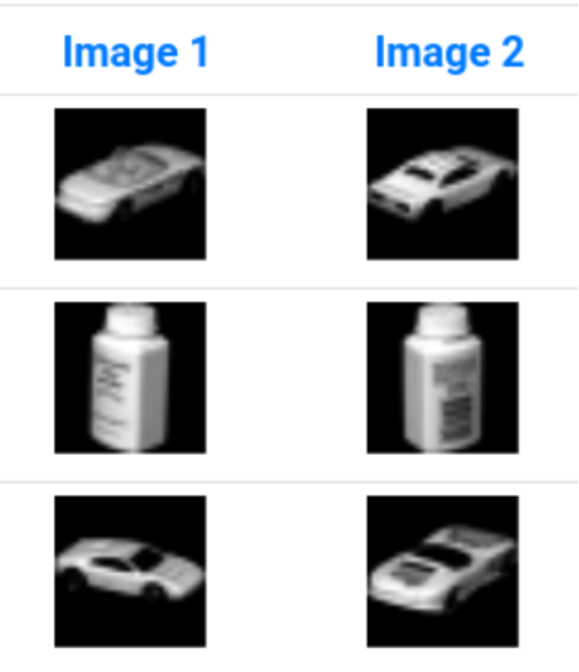
\includegraphics[width=\textwidth]{ml_examples}
        \caption{Similar-link constraints.}
    \end{subfigure}
    \begin{subfigure}[c]{0.48\linewidth}
        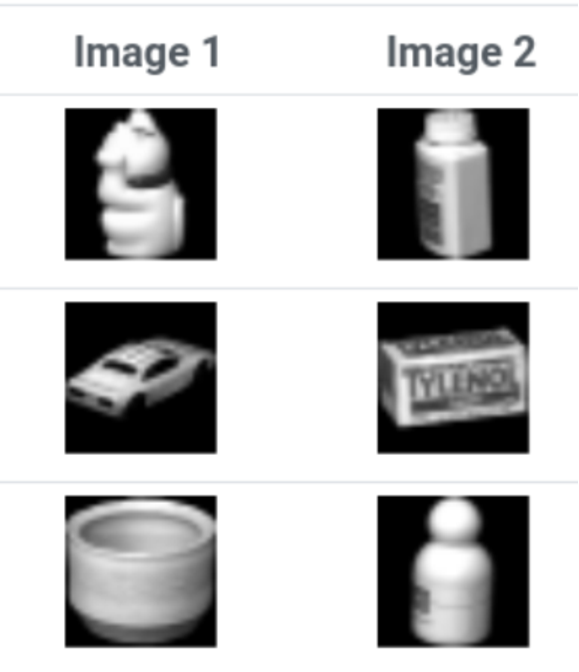
\includegraphics[width=\textwidth]{cl_examples}
        \caption{Dissimilar-link constraints.}
    \end{subfigure}
    \caption{Examples of similar-link and dissimilar-link constraints between pairs of images from COIL20 dataset (a dataset of 20 object captures under many different vantage points).}
    \label{fig:ml_cl_examples}
\end{figure}

Our method is based on the following hypothesis: an embedding is said to be good if it accurately represents the high-dimensional data and satisfies the user constraints. The pairwise constraints can then be used as a criterion to fit the user requirements.
Our method frees users from manually selecting the hyperparameter of $t$-SNE and provides a good quality embedding while preserving their predefined constraints.
To prove the reliability of this hypothesis, we transform the pairwise constraints to a quantitative score (defined in Section~\ref{subsec:s_score}) and compare it with several embedding quality metrics (presented in Section~\ref{subsec:metric}).
More details about the user integration for constraint selection is presented in the next sections.

\subsection{Quantifying the User Constraints}\label{subsec:s_score}
Given an embedding result and a set of user pairwise constraints, our method outputs a score measuring how well the pairwise constraints are preserved in the output embedding, called \emph{constraint-preserving score} $S$.

\subsubsection*{Constraint measurement}
$t$-SNE uses the Student's $t$-distribution to encode the neighborhood information of the instances in the low dimensional space (see Eq.~\ref{eq:q_ij}).
We also use a $t$-distribution in the embedded space to quantify the user constraints preservation.
Let us denote the embedding result of $t$-SNE ${Y} = \{{y_i}\}$, a set of similar-links $\mathcal{M}$ and a set of dissimilar-links $\mathcal{C}$. The number of similar-link and dissimilar-link constraints are denoted by $|\mathcal{M}|$ and $|\mathcal{C}|$, respectively.
For a constrained pair $(i, j)$, the probability of $i$ and $j$ being neighbors is defined as
\begin{equation}\label{equ:q_link}
    q_{ij} = \frac
    { ( 1 + || y_i - y_j ||^2 )^{-1} }
    { \sum_{k \neq l} { ( 1 + ||y_k - y_l||^2 )^{-1} } }.
\end{equation}
The points connected by a similar-link constraint are considered as neighbors and should be close together.
The constrained points in a dissimilar-link should stay apart since they can not be neighbors of each other.
Therefore, for each similar-link $(i,j) \in \mathcal{M}$, $q_{ij}$ should be high and inversely, $q_{ij}$ is expected to be low for each dissimilar-link $(i,j) \in \mathcal{C}$.

\subsubsection*{Constraint-preserving score for similar-links}
The amount of similar-link information preserved in a given embedding is measured as a log-likelihood of the joint distribution of $q_{i j}$ over all similar-links $(i, j) \in \mathcal{M}$:
\begin{equation}
S_{\mathcal{M}} = \frac{1}{|\mathcal{M}|} \log \prod_{(i,j) \in \mathcal{M}} q_{ij}
                = \frac{1}{|\mathcal{M}|} \sum_{(i,j) \in \mathcal{M}} \log q_{ij}.
\end{equation}
If all pairs connected by similar-links are placed close together, the log-likelihood is high and $S_{\mathcal{M}}$ is maximized.

\subsubsection*{Constraint-preserving score for dissimilar-links}
In contrast to similar-links, the probability $q_{ij}$ for each dissimilar-link $(i,j) \in \mathcal{C}$ should be low, i.e. the log-likelihood over all dissimilar-link pairs ($\log \prod_{\mathcal{C}} q_{ij}$) has to be minimized. Or in other words, the negative log-likelihood over all dissimilar-link constraints should be maximized. The constraint-preserving score for a set of dissimilar-links $\mathcal{C}$ is defined as
\begin{equation}
S_{\mathcal{C}} = -\frac{1}{|\mathcal{C}|} \log \prod_{(i,j) \in \mathcal{C}} q_{ij}
                = -\frac{1}{|\mathcal{C}|} \sum_{(i,j) \in \mathcal{C}} \log q_{ij}.
\end{equation}
By maximizing $S_{\mathcal{C}}$, the embedding that respects the best the dissimilar-link constraints is found.
Another way to measure how well a dissimilar-link $(i,j)$ is preserved is to use $1 - q_{ij}$. However, in practice, the value of $q_{ij}$ is very small, which means that $1 - q_{ij}$ is very close to one which makes the log-likelihood of all dissimilar-links vanish.

\subsubsection*{Constraint-preserving score for similar-links and dissimilar-links}

\begin{figure}
    \centering
    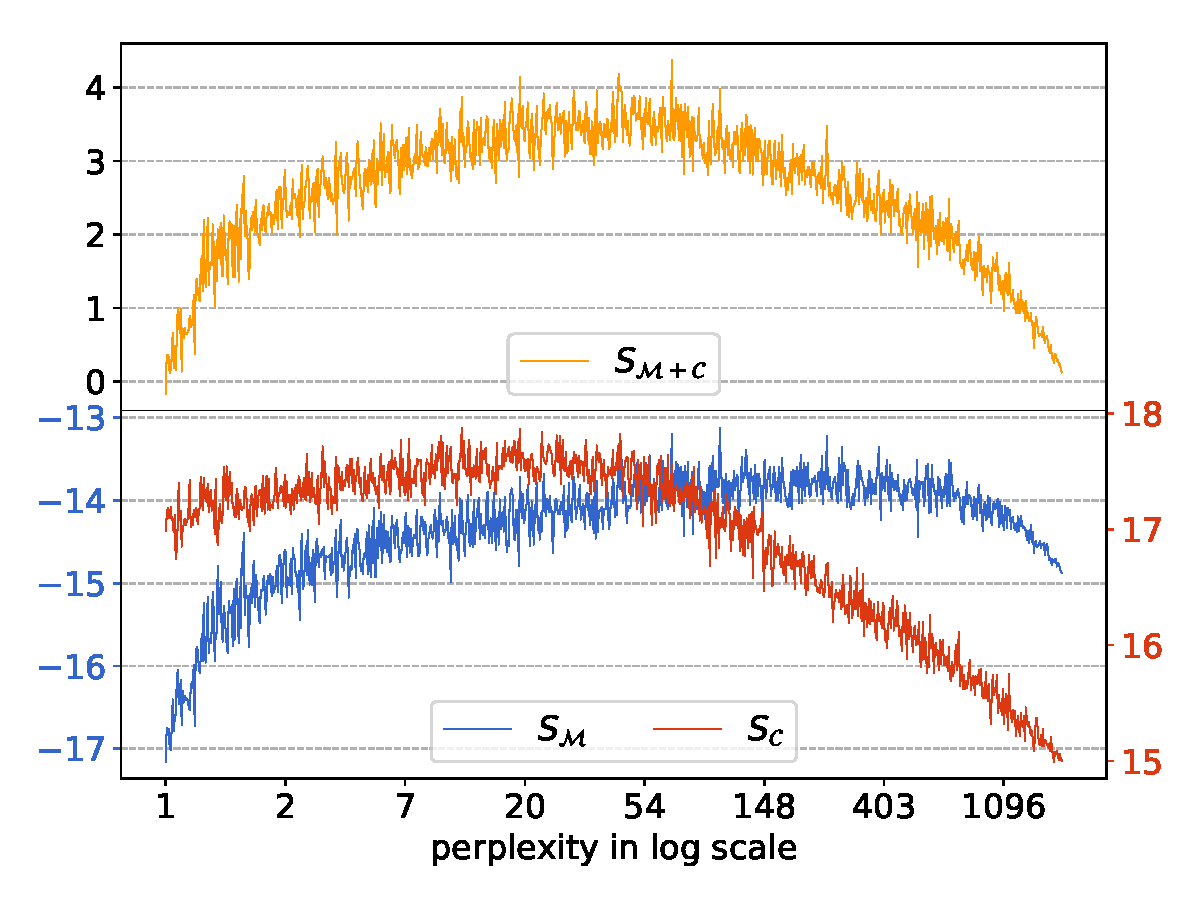
\includegraphics[width=0.85\linewidth]{s_scores_50}
    \caption{[TODO: Replace]Evolution of constraint-preserving scores $S_{\mathcal{M}+\mathcal{C}}$, $S_{\mathcal{M}}$ and $S_{\mathcal{C}}$ with 50 constraints for \emph{DIGITS} over different perplexities.}
    \label{fig:s_scores_mnist}
\end{figure}

The score over all similar-links and dissimilar-links can be maximized at the same time by defining the constraint-preserving score as a combination with equal contribution of both $S_{\mathcal{M}}$ and $S_{\mathcal{C}}$, i.e. $S_{\mathcal{M}+\mathcal{C}} = S_{\mathcal{M}} + S_{\mathcal{C}}$.

An embedding that retains as much as possible the constraint information is considered to have a good quality with respect to the user needs.
Based on these definitions, our method takes a set of user-defined pairwise constraints and searches among all embeddings created by different perplexities for one with maximal $S_{\mathcal{M}+\mathcal{C}}$.
Fig.~\ref{fig:s_scores_mnist} illustrates the contribution of $S_{\mathcal{M}}$ and $S_{\mathcal{C}}$ to the overall $S_{\mathcal{M}+\mathcal{C}}$ score for \emph{DIGITS} dataset with 50 auto-generated constraints (see Section~\ref{subsec:constraint_preparation} for details about the generation process).

Let us recall how the structure of the visualization changes according to perplexity values, such as shown in Fig.~\ref{fig:mnist_perps}.
First, when the perplexity is very small, only a small number of neighbors is considered for each point. Hence, instances in the visualization seems like randomly drawn from a uniform distribution (see perplexity=1 in Fig.~\ref{fig:mnist_perps}). In this case, it is unlikely that similar-link constraints are preserved, which leads to very low value of $S_{\mathcal{M}}$. In contrast, $S_{\mathcal{C}}$ should be very high as it is likely that different instances are further apart, meaning that dissimilar-links are well preserved. These high $S_{\mathcal{C}}$ value and low $S_{\mathcal{M}}$ value is what can be observed for small perplexity in the left part of Fig.~\ref{fig:s_scores_mnist}.
Second, when the perplexity increases, more neighbors are considered for each point and compact clusters are formed. This facilitates the preservation of similar-links, as similar instances are more and more close together, and makes it difficult for dissimilar-links to be preserved.
This explains why we observe the increase of $S_{\mathcal{M}}$ and the decrease of $S_{\mathcal{C}}$ when the perplexity increases.
Finally, when the perplexity is too large (when almost every point is neighbor to each other), the visualization becomes a very dense cluster (see more examples in Fig.~\ref{fig:meta_mnist}, \ref{fig:meta_coil}, \ref{fig:meta_breast_cancer} and \ref{fig:meta_country}), which makes $S_{\mathcal{C}}$ decreasing drastically.
By combining similar-link and dissimilar-link constraints with an equal contribution, $S_{\mathcal{M}+\mathcal{C}} = S_{\mathcal{M}} + S_{\mathcal{C}}$ discourages both too small and too large perplexities.

\subsection{Visualization Quality Metrics for Evaluation}\label{subsec:metric}
There exist several metrics to evaluate the quality of an embedding. This section presents five of these metrics that we use for evaluating the embedding selected by our proposed method. 
In this paper, among the possible quality measures, we do not consider clustering quality measures because cluster metrics need labeled data for measurement (e.g. the image-related number in the dataset MNIST), which would restrict the datasets on which we can evaluate the user constraints approach.
For these reasons, we only use cluster-label agnostic metrics to measure the quality of the $t$-SNE embeddings.
We also avoid quality measures that are linked to the objective function of SNE, e.g. Neighborhood Retrieval Visualizer (NeRV) \cite{venna2010}, (i) because they need the evaluation of their (own) perplexity parameter and (ii) because of the bias of measuring the quality of $t$-SNE with a quality metric too closely related to SNE.

\begin{table}
\renewcommand{\arraystretch}{1.08}
\caption{Properties of the five cluster-label-agnostic quality metrics considered in this paper to assess visualizations.}\label{tab:metrics}
\begin{tabular}{c c p{4.5cm}}
\hline
Metric name &  Range value & Description\\
\hline \hline
CC & $[0, 1]$ & Pearson correlation coefficient between pairwise distance vectors\\
NMS & $[0, +\infty)$ & Stress based on comparison of pairwise distance orders\\
CCA & $[0, +\infty)$ & Stress with accent put on low dim.\\
NLM & $[0, +\infty)$ & Stress with accent put on high dim.\\
AUC$_{log}$RNX & $[0, 1]$ & How neighbors in high dim. are preserved in low dim.\\
\hline
\end{tabular}
\end{table}

Five metrics have been selected for evaluating the quality of visualizations. 
The first considered metric, the \emph{correlation coefficient} (CC)~\cite{geng2005}, compares the pairwise distances in the HD and LD spaces by computing the correlation between the distance vectors in HD and LD. The well-known \emph{Kruskal's non-metric stress} (NMS)~\cite{kruskal1964}, often used as objective function of non-metric multidimensional scaling, is used to compare the pairwise distance orders between the high and low-dimensional space. The \emph{curvilinear component analysis stress}~(CCA) \cite{demartines1997} is a kind of Kruskal's stress with an emphasis on the embedding pairwise distances. The metric evaluates the embedding quality by looking if instances in the low-dimensional space are close to each other. The \emph{Sammon's non-linear mapping stress}~(NLM)~\cite{sammon1969}, is a measure similar to CCA, but focusing on the closeness of instances in the high-dimensional space. Finally, the \emph{AUC$_{log}$RNX}~\cite{lee2015} compares the neighborhood of each instance in the high and low-dimensional spaces for all possible neighborhood sizes. Table~\ref{tab:metrics} summaries these metrics and mathematical details are provided in Appendix A. %~\ref{appendix:qual_metrics}.

The quality metrics considered here are used to control the change in quality when varying the perplexity. How we precisely compare these metrics with the constraint-preserving scores is presented in the next section.

%%%%%%%%%%%%%%%%%%%%%%%%%%%%%%%%%%%%%%%%%%%%%%%%%%%%%%%%%%%%%%%%%%%%%%%%%%%%%%
% FIX LAYOUT
% \begin{figure*}
%     \centering
%     \includegraphics[width=0.92\linewidth]{app_guis_annotated}
%     \caption{User interface for constraint selection with an image dataset (\emph{COIL20} - on the left) and with a multivariate dataset (\emph{COUNTRY2014} - on the right).
%     (A) Drop-down menu for selecting the dataset and some details about the number of instances and features for the selected dataset.
%     (B1) A pair of images are shown for comparing.
%     (B2) Two multivariate examples are shown in radar chart. To easily compare them, only distinguishable features are presented.
%     (C) Control buttons allow user to decide whether a pair is a similar-link or a dissimilar-link. The user can ignore the current pair and jump to next pair by clicking \emph{"Next"}, reset the current interactive session by clicking \emph{"Reset"}, or save the selected constraints and terminate the session by clicking \emph{"Done"}.
%     (D) List of selected similar-link and dissimilar-link constraints in the current session.}
%     \label{fig:app_gui}
% \end{figure*}

\section{Experimental setup}\label{XP}
This section presents a way to select the pairwise constraints proposed in Section~\ref{subsec:s_score} to express user requirements, as well as the evaluation of our proposed method.
First, the datasets used in our experiments are presented in Section~\ref{subsec:dataset}. Second, an initialization strategy for running $t$-SNE efficiently multiple times is introduced in Section~\ref{subsec:chained-t-SNE}.
Third, the interface for selecting constraints is detailed in Section~\ref{subsec:constraint_preparation}.
Finally, Section~\ref{subsec:protocol} presents the overall protocol for evaluating the constraint-preserving scores.

\subsection{Datasets}\label{subsec:dataset}

\begin{table}[h]
\renewcommand{\arraystretch}{1.08}
\centering
\begin{tabular}{l p{1.5cm} p{1.5cm} p{1.5cm}}
\hline
Dataset name & \# instances & \# features & \# classes \\
\hline\hline
\emph{DIGITS} & 1797 & 64 & 10\\
\emph{COIL20} & 1440 & 1024 & 20\\
\emph{FASHION} & 200 & 784 & 10\\
\emph{COUNTRY 2014} & 246 & 140 & 6 \\
%\emph{BREAST-CANCER} & 569 & 30 & 2\\
% \emph{MPI} & 99 & 6 & 9\\
%\emph{DIABETES} & 768 &  8 & 2\\
\hline
\end{tabular}
\caption{Description of the datasets used for the evaluation.}
\label{tab:dataset}
\end{table}

For evaluating the proposed perplexity selection strategy, several well-know datasets are used. They have the particularity of either containing images or instances that can be identified by a label (e.g. country names). The reason behind this choice is that for users to know how to put constraints on instance pairs, he first has to identify those instances. 
\emph{DIGITS}~\cite{Dua2017} is a dataset of hand-written digits in which each instance is an 8x8 gray-scale image.
\emph{COIL20} \cite{nene1996} is a dataset of 32x32 gray-scale pictures of 20 rotated objects.
\emph{COUNTRY2014} \cite{world2014} is the World Development Indicators dataset that contains indicators for countries and economic centers in the world in 2014.
%\emph{BREAST-CANCER} \cite{Dua2017}, Breast Cancer Wisconsin Diagnostic, is a dataset containing 357 benign and 212 malignant breast cancer instances.
\emph{MPI} \cite{alkire2017} is a Multidimensional Poverty Measures dataset that indexes different types of simultaneous deprivation in 99 countries.
%\emph{DIABETES} \cite{Dua2017}, Pima Indians Diabetes is a dataset on the onset of diabetes based on diagnostic measures.  
%Fashion dataset: https://github.com/zalandoresearch/fashion-mnist
\emph{FASHION} \cite{xiao2017/online} is a dataset containing 28x28 images of fashion products. 
The characteristics of the datasets used in our experiments are summarized in Table~\ref{tab:dataset}. Class labels for all used datasets are available, but they are not used for calculating embeddings by $t$-SNE, nor for computing the quality metrics.

\subsection{Constraints Selection Interface}\label{subsec:constraint_preparation}

\begin{figure*}
    \centering
    \includegraphics[width=\linewidth]{Demo_app.png}
    \caption{Interactive interface allowing users to select dissimilar links (red lines) between instances, as well as similar links (green lines). In order to draw these constraints, the user select two instances in the central visualization, and hit the button ``Similar'' or ``Dissimilar''. When the selection is finished, the user can click on the ``Find best viz'' button in order for the visualization to change according to the constraints. On the right, the constraint scores and the quality metrics scores are presented for all perplexity values in log scale.}\label{fig:app_gui}
\end{figure*}

To facilitate the constraint selection, an interface (see Fig.~\ref{fig:app_gui}) is introduced that allows users to link some instances based on their similarity or dissimilarity in order to form the pairwise similar-link or dissimilar-link constraints. Users can propose similar and dissimilar constraints by selecting pairs of instances in the central visualization and hitting the ``Similar'' or ``Dissimilar'' button on the left. When users are finished with the selection, they can hit the ``Find best viz'' button, which will choose another perplexity such that the visualization best correspond to $S_{\mathcal{M}+\mathcal{C}}$. In order to enable such selection, users must be able to identify the instances, which is why we restricted our datasets to the ones containing images and instance names (e.g. country names). A zoom has been implemented to handle the case of crowded regions in the visualization, or if the number of instances is too high to allow users to easily pick out pairs of instances in the visualization.

\subsection{Evaluation Protocol}\label{subsec:protocol}

First of all, we want to know the contribution of each type of user constraint to the constraint-preserving score. Therefore, we calculate $S$ with only similar-links $S_{\mathcal{M}}$, only dissimilar-links $S_{\mathcal{C}}$ and with both of them $S_{\mathcal{M+C}}$. 
In order to analyze the effect of the number of constraints on $S$, different numbers of constraints are used to calculate $S$ for each dataset. 
% For a fixed number of constraints, the constraint generation process is repeated 10 times in order to generate different constraint pairs.
The goal of our experiments is to compare the visualization with a perplexity selected by $S$ with the quality metrics mentioned in Section~\ref{subsec:metric}. 
In other words, for each dataset we investigate the link between the constraint preserving scores $S$ and the quality metric scores over different perplexities. 
The evaluation for each dataset is done through the following steps:
\begin{enumerate}[leftmargin=*]
  \item Predefine a list of perplexity in log-scale and calculate the embeddings for each perplexity based on Chained-$t$-SNE.  Chained-$t$-SNE is based on the $t$-SNE implementation of \textit{scikit-learn}\cite{scikit-learn}.
  \item Calculate the constraint-preserving scores $S_{\mathcal{M+C}}, S_{\mathcal{M}}, S_{\mathcal{C}}$ for each embedding with different number of constraints.
  \item Calculate the five quality metrics for each embedding. Notice that for the two bounded metrics $AUC_{log}RNX$ and $CC$, the higher value, the better embedding quality, and for the three unbounded metrics ($NMS$, $CCA$, $NLM$), best values are close to zero. For consistency with constraint-preserving scores and bounded-metric scores, we use the opposite values of the unbounded metrics.
  \item Calculate the Bayesian information criterion-based score proposed by Cao and Wang~\cite{cao2017automatic}. In that work, small values of \emph{BIC} score are preferred. For consistency with the above scores, we take the opposite value of \emph{BIC} scores and therefore prefer large values.
  \item The constraint-preserving scores are compared with the quality metric scores and with the \emph{BIC}-based scores by using the \textit{cosine distance}, a measure of similarity between two series of values. The \textit{cosine distance} is in the range $[0,2]$, $0$ for two similar series and $2$ for two different series.
\end{enumerate}
A comparative result of cosine distances between the scores defined in our experiments is detailed in Section~\ref{subsec:result_compare}.

%%%%%%%%%%%%%%%%%%%%%%%%%%%%%%%%%%%%%%%%%%%%%%%%%%%%%%%%%%%%%%%%%%%%%%%%%%%%%%
\section{Results}\label{sec:results}
In this section, the results of our experiments are presented to answer the research question stated in the introduction: is the constraint-preserving score reliable and how good are visualizations with respect to well-known visualization quality metrics?

\subsection{Characteristics of the constraint-preserving scores}\label{subsec:result_s_score}

\begin{figure}
  \centering
  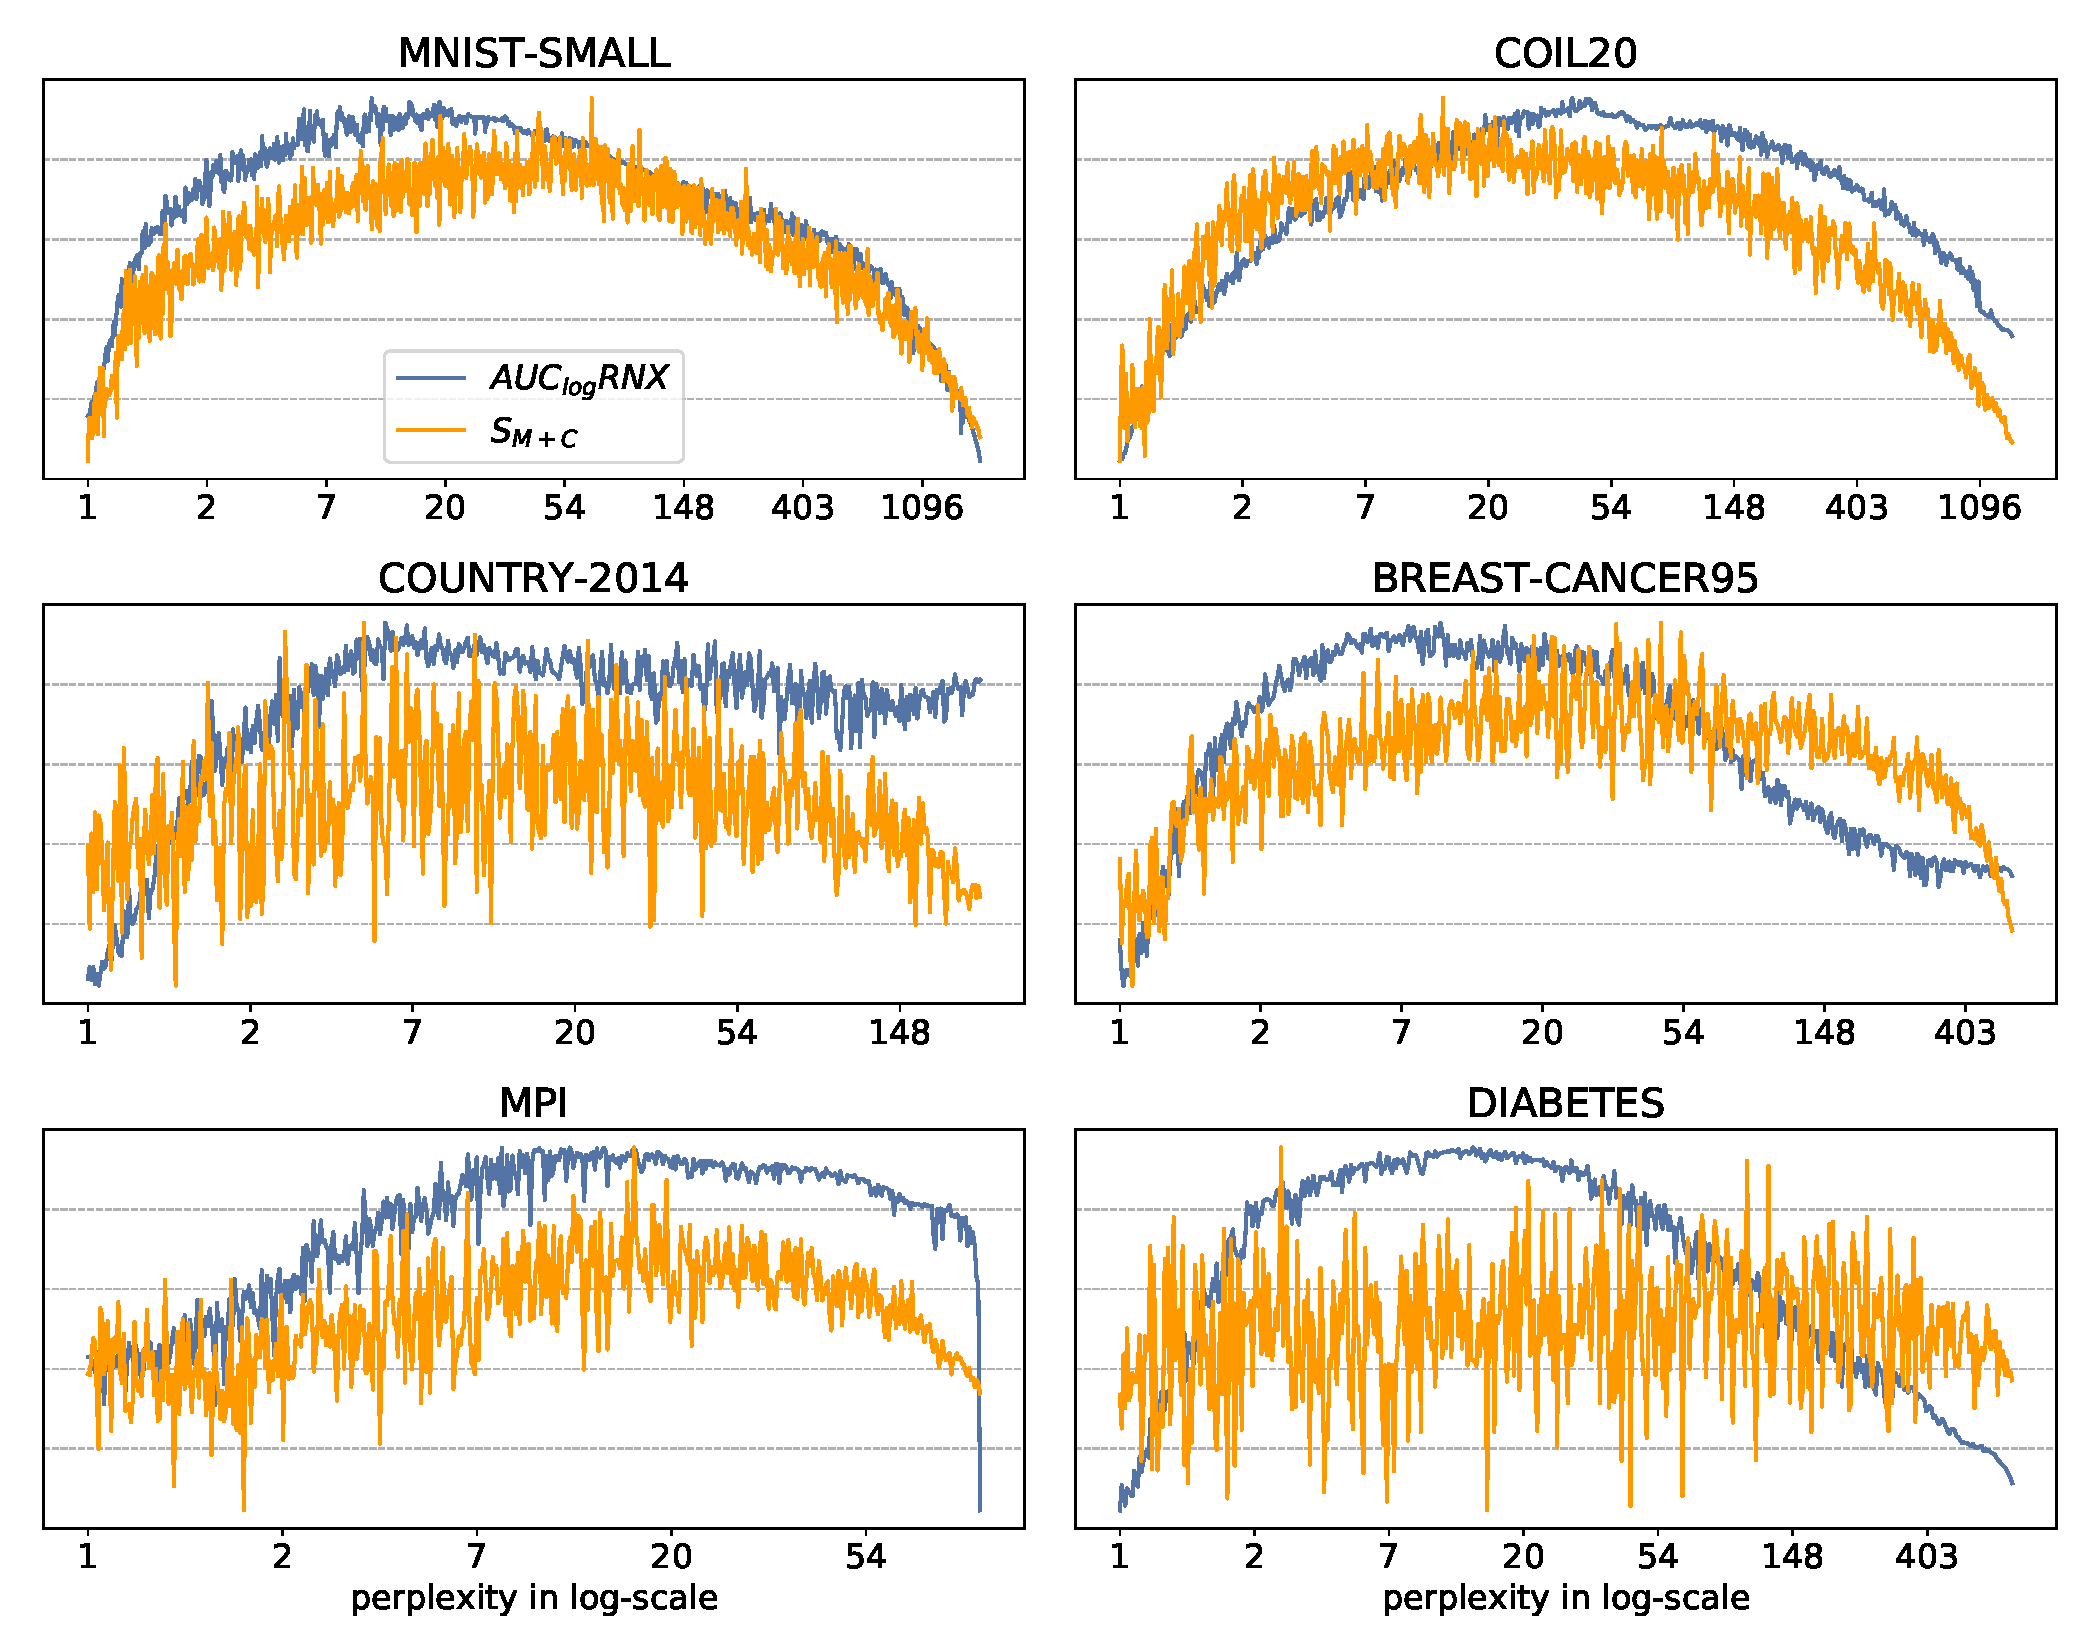
\includegraphics[width=\linewidth]{sall_auc_50}
  \caption{Similarity between $S_{\mathcal{M}+\mathcal{C}}$ and $AUC_{log}RNX$.}
  \label{fig:compare_sall_auc}
\end{figure}

Our most important result concerns the relation between the constraint-preserving scores and the perplexity of $t$-SNE. 
The constraint-preserving score $S_{\mathcal{M}+\mathcal{C}}$ over different number of constraints roughly has a convex form with respect to the perplexity value. This can be seen in Fig.~\ref{fig:compare_sall_auc}, which shows an example with 50 of each similar-link and dissimilar-link constraints. This convex form assures that we can find the optimal perplexity regarding $S_{\mathcal{M}+\mathcal{C}}$.%, meaning a value for which $S_{\mathcal{M}+\mathcal{C}}$ reaches its maximum.

\begin{figure}
    \centering
    \includegraphics[width=\linewidth]{sall_perp20}
    \caption{The constraint-preserving score $S_{\mathcal{M}+\mathcal{C}}$ with different number of constraints. The $t$-SNE embeddings are calculated with a perplexity of 20. The bar chart shows the average values and the vertical thin lines represent the standard deviations of $S_{\mathcal{M}+\mathcal{C}}$.}
    \label{fig:s_nconstraint}
\end{figure}

From the Fig.~\ref{fig:compare_sall_auc}, we can see that $S_{\mathcal{M}+\mathcal{C}}$ has a large distortion for \emph{COUNTRY2014} and \emph{DIABETES} datasets.
The effect of the number of constraints on the constraint-preserving scores is analyzed in order to understand the reason of this instability.
We take all embeddings with a perplexity of 20 for all six datasets, and then calculate $S_{\mathcal{M}+\mathcal{C}}$ with different number of constraints (from few to hundreds of constraints).
Fig.~\ref{fig:s_nconstraint} shows that, for all dataset, a small number of constraints (1, 2 or 5) leads to a large variance.
For the \emph{COUNTRY2014} and \emph{DIABETES} datasets, $S_{\mathcal{M}+\mathcal{C}}$ always has a large variance, which provokes the unstable results shown in Fig.~\ref{fig:compare_sall_auc}. 
For the four other datasets, from 10 of each similar-link and dissimilar-link constraints, $S_{\mathcal{M}+\mathcal{C}}$ becomes consistently stable. Other perplexity values of perplexity provide similar results.%, mainly with the three datasets \emph{DIGITS}, \emph{COIL20} and \emph{BREAST-CANCER95}.

\subsection{Comparison with the \emph{BIC}-based Score and the Quality Metric Scores}\label{subsec:result_compare}

\begin{figure*}
    \centering
    \includegraphics[width=0.95\linewidth]{cosine_distance_50}
    \caption{Cosine distances between the constraint-preserving scores, the five metric scores and the \emph{BIC}-based score. A cosine distance of 0 means that the scores are similar and $2$ means that they are completely dissimilar.}
    \label{fig:cosine_dist}
\end{figure*}

As presented in the experimental protocol in Section~\ref{subsec:protocol}, the constraint-preserving scores $S$ are compared with the \emph{BIC}-based score and five quality metric scores by using the cosine distance. % that takes a value in the range $[0,2]$. 
A comprehensive comparison for all six datasets is made in Fig.~\ref{fig:cosine_dist}.
If the cosine distance is close to zero, $S$ will be close to a metric or to the \emph{BIC} score.
Otherwise, if the cosine distance is close to two, $S$ will be different from a metric or the \emph{BIC} score.
The constraint-preserving scores in this comparison are calculated with 50 of each similar-link and dissimilar-link constraint type.
Some observations from this experiment should be highlighted.

First, $S_{\mathcal{M}+\mathcal{C}}$ is very similar to the $AUC_{log}RNX$ metric score, as it can also be seen in Fig.~\ref{fig:compare_sall_auc}. This echoes Bibal et al. who show that $AUC_{log}RNX$ scores correspond to visualizations preferred by users \cite{bibal2016}. This can be due to the fact that pairwise constraints implicitly reflect the neighborhood information and thus agree with the neighborhood-preserving criteria of $AUC_{log}RNX$.

\begin{figure}
  \centering
  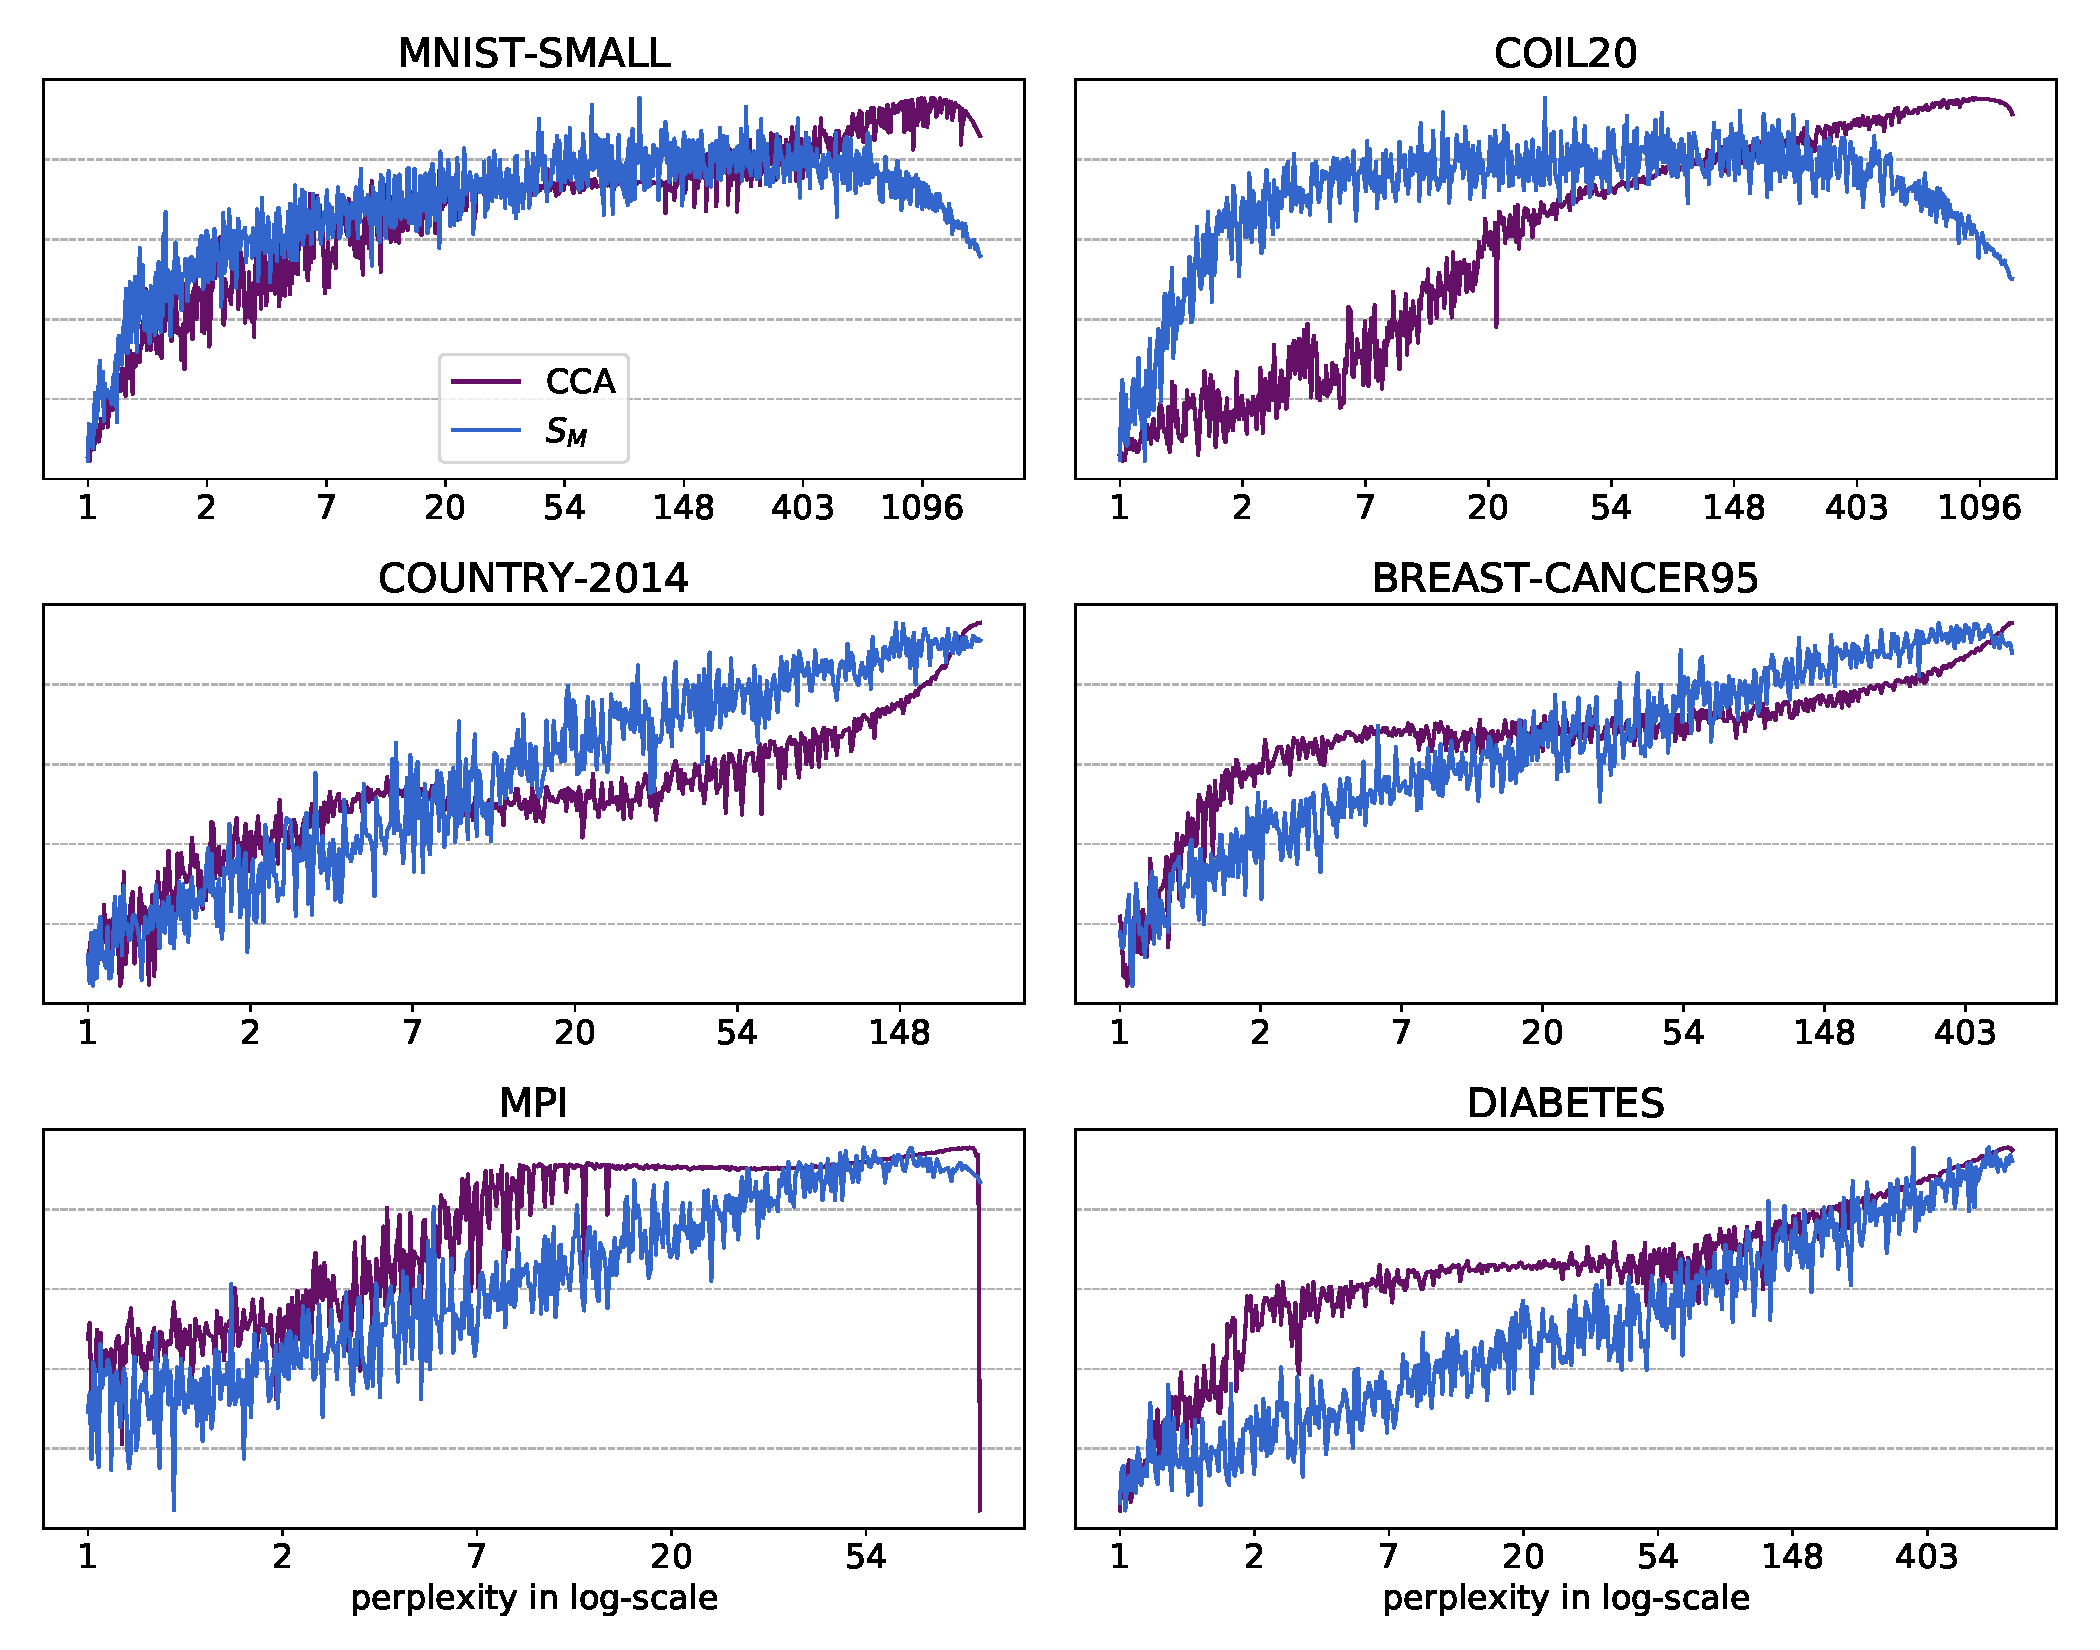
\includegraphics[width=\linewidth]{sml_cca_50}
  \caption{Similarity between $S_{\mathcal{M}}$ and $CCA$.}
  \label{fig:compare_sml_cca}
\end{figure}

Second, $S_\mathcal{M}$ is close to almost every other presented metrics, meaning $CC$ and the three unbounded stress-based metrics $NMS$, $NLM$ and $CCA$.% For instance, $NLM$ focuses on the closeness of instances in LD while $CCA$ focuses on the closeness in HD. $S_{\mathcal{M}}$, the similar-link preserving score, agrees the most with these metrics. 
Fig.~\ref{fig:compare_sml_cca} shows a comparison between $S_\mathcal{M}$ and $CCA$. The $CCA$ score consistently increases when the perplexity increases. Since the embedding tends to be more compact when the perplexity is large, the closeness is more likely to be preserved. $S_{\mathcal{M}}$ also prefers embeddings with compact clusters, as it encourages similar-link constraints preservation.

\begin{figure}
  \centering
  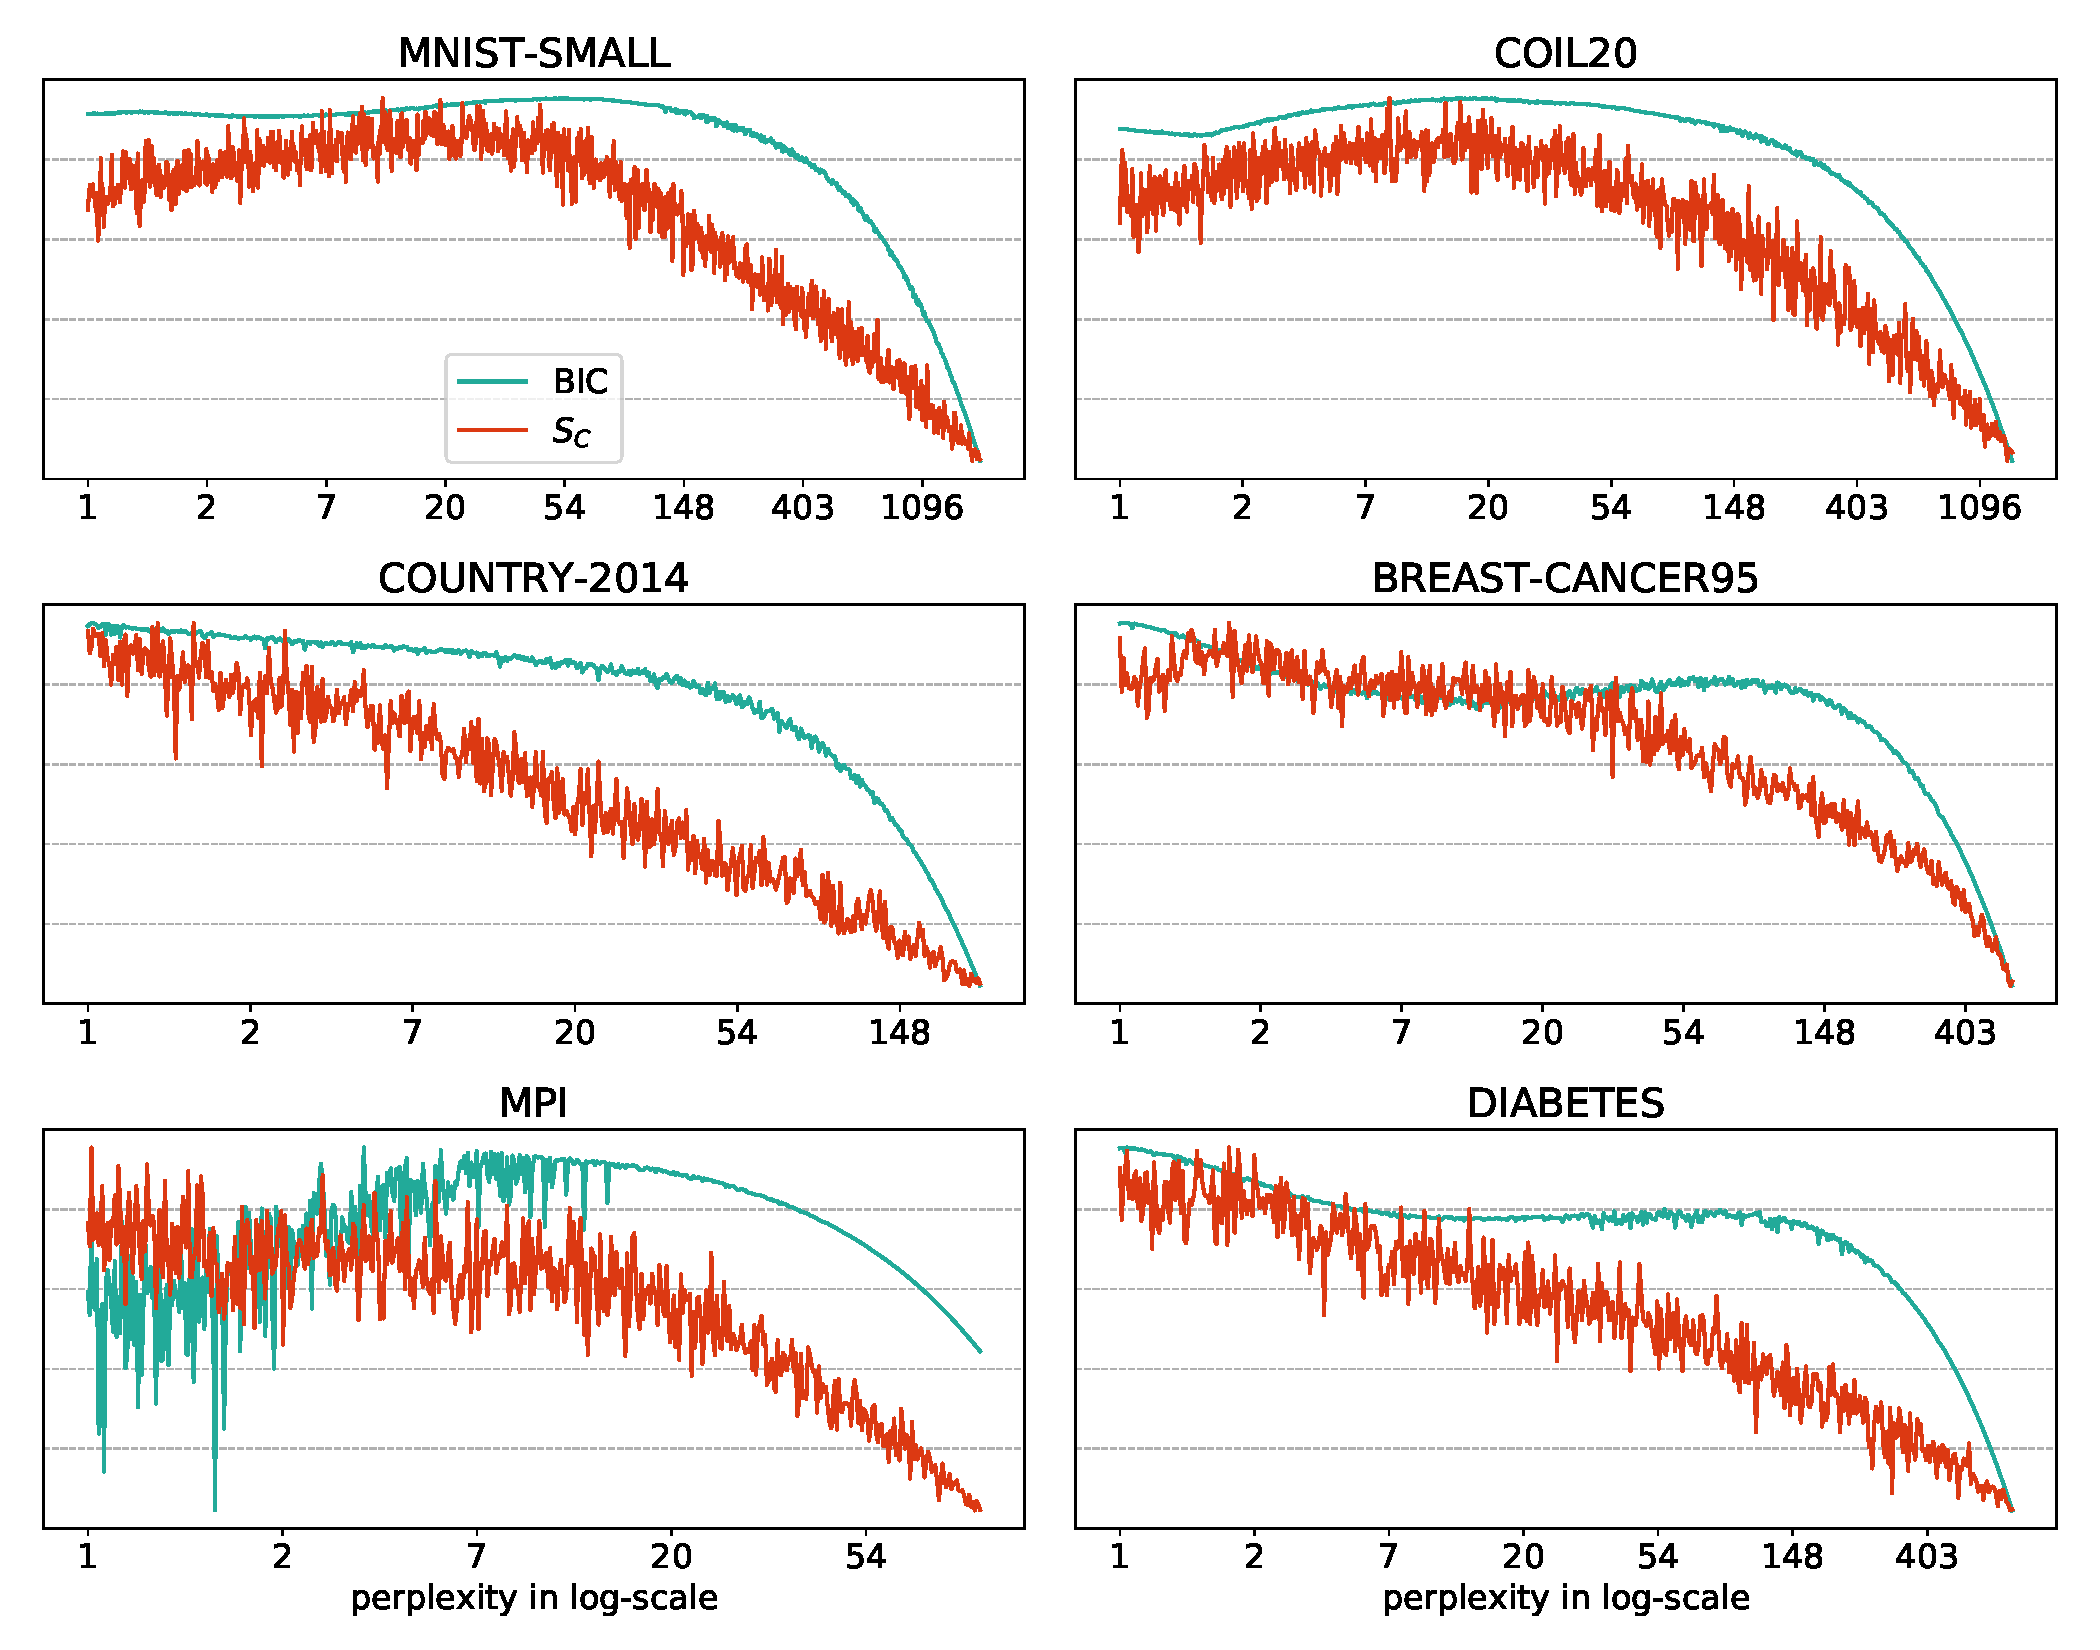
\includegraphics[width=\linewidth]{scl_bic_50}
  \caption{Similarity between $S_{\mathcal{C}}$ and the $BIC$-based score.}
  \label{fig:compare_scl_bic}
\end{figure}

Finally, $S_\mathcal{C}$ seldom agrees with any quality metric but consistently agrees with the \emph{BIC} score (see Fig.~\ref{fig:compare_scl_bic}). This may be explained by the fact that the \emph{BIC}-based score tends to prefer small perplexities, which corresponds to the constraint-preserving score $S_\mathcal{C}$ with only dissimilar-links.

%When the pairwise constraints are available, the proposed constraint-preserving scores are considered more general than the quality metrics and the \emph{BIC}-based score for selecting the best visualization.
The comparison results can be summed up as follow. 
If only similar-link constraints are used, we end up with similar results as when using $CC$ or the unbounded metric scores.
If only dissimilar-link constraints are used, we end up with similar results as using the \emph{BIC}-based score.
When both types of constraint are combined, the obtained results correspond to $AUC_{log}RNX$.
The visualization of the best embeddings selected by all presented scores are shown in the following section.

\subsection{Best Visualizations for all Methods}\label{subsec:result_viz}


TODO: Should selected candidates of BO in the metamap.


In order to show all visualizations created by the perplexities selected using the different metrics, \emph{meta-maps} of all embeddings for each dataset are presented in Fig.~\ref{fig:meta_mnist}, Fig.~\ref{fig:meta_coil}, Fig.~\ref{fig:meta_breast_cancer} and Fig.~\ref{fig:meta_country}.
A meta-map is a visualization of embeddings, which makes it easier to discover the similarity between the different selections.
A gentle introduction and application of meta-maps can be found in \emph{VisCoDeR}~\cite{cutura2018viscoder}.
The precalculated embeddings corresponding to each perplexity are used as features to construct the meta-map with $t$-SNE. This meta-map helps us to discover the local relationship (or similarity) between the embeddings.
Each point in the meta-map corresponds to an embedding and is colorized by perplexity value in log-scale.

With meta-maps, one can easily find separated clusters of embeddings with high and low perplexities.
The best visualization according to the three constraint-preserving scores, the five quality metrics and the \emph{BIC}-based score are marked.
The visualization of the best embeddings found by $S$, by the quality metrics and the \emph{BIC}-based score are shown for comparison.
In most cases, $CC$, $CCA$, $NMS$ and $NLM$ give approximately the same perplexity value, which is often too large. However the visualization corresponding to a large perplexity value is always a crowded cloud without clear structure, which could not be considered as a good embedding. In contrast, in the best embeddings found by $AUC_{log}RNX$ and the three constraint-preserving scores, hidden patterns in the datasets can be easily recognized.

Fig.~\ref{fig:meta_mnist} and Fig.~\ref{fig:meta_coil} present, in meta-maps, the best embeddings selected based on 50 of each type of similar-link and dissimilar-link for the \emph{DIGITS} and \emph{COIL20} datasets.
We also demonstrate the usefulness of user constraints with two multivariate datasets \emph{BREAST-CANCER} and \emph{COUNTRY2014}.
10 similar-links and 10 dissimilar-links are manually selected via the graphical interface shown in Fig.~\ref{fig:app_gui}. The meta-maps, along with the best embeddings for these two datasets, are shown in Fig.~\ref{fig:meta_breast_cancer} and Fig.~\ref{fig:meta_country}.

%%%%%%%%%%%%%%%%%%%%%%%%%%%%%%%%%%%%%%%%%%%%%%%%%%%%%%%%%%%%%%%%%%%%%%%%%%%%%%
\section{Discussion and Conclusion}\label{sec:ccl}

In this work, we consider user knowledge under the form of constraints in order to find the most suitable visualization for him. A user constraint-based method is proposed to select the perplexity, an important hyperparameter of $t$-SNE. By searching through different perplexity values, we can select the one for which the corresponding embedding satisfies the given pairwise user constraints the most.
For several datasets, we show that only 10 user pairwise constraints of each type, similar-link and dissimilar-link, are sufficient for generating quality embeddings.
This result suggests that we can automate the process of selecting the hyperparameter for $t$-SNE, the perplexity, based on user constraints instead of observing many embedding scatter plots.
The constraints can be collected via an interactive interface, in which the user can freely decide the similarity between pairs of visual objects. In order to make it possible to run many $t$-SNE with a low computational cost, Chained-$t$-SNE has been presented. 
%The natural cognitive recognition ability of users is used to form the constraints without requiring any domain expert knowledge about the studied dataset.

The embedding found by our method is also one of the best embeddings with respect to $AUC_{log}RNX$, the state-of-the-art NLDR quality metric.
Moreover, calculation of constraint-preserving scores is simpler than other sophisticated metrics.
From our experimental results, we also show that each constraint-preserving score can agree with one or more of the five quality measures or the \emph{BIC}-based score. More specifically, $S_{\mathcal{M}+\mathcal{C}}$ is close to $AUC_{log}RNX$ metric, $S_{\mathcal{M}}$ is close to the unbounded stress-based metrics and $S_{\mathcal{C}}$ is similar to the \emph{BIC}-based score.

The most important contribution of our work is to make complex visualization technique like $t$-SNE accessible to users by freeing them from the tedious task of selecting the hyperparameter.
%We need, however, to precalculate the embeddings with many perplexity values.
%The perspective for our future work is to find a more dynamic way to select the best perplexity without performing a search over many values. Furthermore, 
A future work is to develop other types of constraints that could capture other forms of user need. 
